\section{Experiments}
\label{sec:experiments}
In this section, we evaluate our approach on two related tasks: visual object tracking (on VOT-2016 and VOT-2018) and semi-supervised video object segmentation (on DAVIS-2016 and DAVIS-2017).
We refer to our \emph{two-branch} and \emph{three-branch} variants with SiamMask-2B and SiamMask respectively.

\subsection{Evaluation for visual object tracking}
\label{sec:exp_track}

\mypar{Datasets and settings.}
We adopt two widely used benchmarks for the evaluation of the object tracking task: VOT-2016~\cite{kristan2016visual} and VOT-2018~\cite{VOT2018}, both annotated with rotated bounding boxes.
We use VOT-2016 to understand how different types of representation affect the performance.
For this first experiment, we use mean intersection over union (IOU) and Average Precision (AP)@$\{0.5,0.7\}$ IOU.
We then compare against the state-of-the-art on VOT-2018, using the official VOT toolkit and the Expected Average Overlap (EAO), a measure that considers both accuracy and robustness of a tracker~\cite{VOT2018}.


\mypar{How much does the object representation matter?}
Existing tracking methods typically predict axis-aligned bounding boxes with a fixed~\cite{bertinetto2016fully,henriques2015tracking,danelljan2015learning,lukezic2017discriminative} or variable~\cite{SiamRPN,held2016learning,zhu2018distractor} aspect ratio.
We are interested in understanding to which extent producing a per-frame binary mask can improve tracking.
In order to focus on representation accuracy, for this experiment only we ignore the temporal aspect and sample video frames at random.
The approaches described in the following paragraph are tested on randomly cropped search patches (with random shifts within $\pm16$ pixels and scale deformations up to $2^{1\pm0.25}$) from the sequences of VOT-2016.


In Table~\ref{tab:iou}, we compare our \emph{three-branch} variant using the \emph{Min-max}, \emph{MBR} and \emph{Opt} approaches (described at the end of Section~\ref{sec:siammask} and in Figure~\ref{fig:bbox}).
For reference, we also report results for SiamFC and SiamRPN as representative of the fixed and variable aspect-ratio approaches, together with three \emph{oracles} that have access to per-frame ground-truth information and serve as upper bounds for the different representation strategies.
(1) The fixed aspect-ratio oracle uses the per-frame ground-truth area and center location, but fixes the aspect reatio to the one of the first frame and produces an axis-aligned bounding box.
(2) The \emph{Min-max} oracle uses the minimal enclosing rectangle of the rotated ground-truth bounding box to produce an axis-aligned bounding box.
(3) Finally, the \textit{MBR} oracle uses the rotated minimum bounding rectangle of the ground-truth.
Note that (1), (2) and (3) can be considered, respectively, the performance upper bounds for the representation strategies of SiamFC, SiamRPN and SiamMask.

Table~\ref{tab:iou} shows that our method achieves the best mIOU, no matter the box generation strategy used (Figure~\ref{fig:bbox}).
Albeit SiamMask-\textit{Opt} offers the highest IOU and mAP, it requires significant computational resources due to its slow optimisation procedure~\cite{vojir2017pixel}. 
SiamMask-\textit{MBR} achieves a mAP@0.5 IOU  of $85.4$, with a respective improvement of $+29$ and $+9.2$ points w.r.t. the two fully-convolutional baselines.
Interestingly, the gap significantly widens when considering mAP at the higher accuracy regime of 0.7 IOU: $+41.6$ and $+18.4$ respectively.
Notably, our accuracy results are not far from the fixed aspect-ratio oracle.
Moreover, comparing the upper bound performance represented by the oracles, it is possible to notice how, by simply changing the bounding box representation, there is a great room for improvement (\eg $+10.6\%$ mIOU improvement between the fixed aspect-ratio and the \textit{MBR} oracles).

Overall, this study shows how the \textit{MBR} strategy to obtain a rotated bounding box from a binary mask of the object offers a significant advantage over popular strategies that simply report axis-aligned bounding boxes.

\begin{table}[t]
\tablestyle{3.5pt}{1.1}
\begin{tabular}{l|x{42}|x{52}x{52}}
 & mIOU  ($\%$) &  mAP@0.5 IOU  &  mAP@0.7 IOU   \\
\shline
Fixed a.r. Oracle  & 73.43 & 90.15  & 62.52   \\
\textit{Min-max} Oracle  & 77.70 & 88.84  & 65.16  \\
\textit{MBR} Oracle & 84.07 & 97.77 & 80.68 \\
\hline
SiamFC~\cite{bertinetto2016fully}  & 50.48 & 56.42  & 9.28   \\
SiamRPN~\cite{zhu2018distractor}  & 60.02 & 76.20  & 32.47  \\
\hline
\bd{SiamMask}-\textit{Min-max} & 65.05 & 82.99  & 43.09 \\
\bd{SiamMask}-\textit{MBR} & 67.15 & 85.42  & 50.86  \\
\bd{SiamMask}-\textit{Opt} & \bd{71.68} & \bd{90.77} & \bd{60.47}
\end{tabular}
\vspace{1mm}
\caption{Performance for different bounding box representation strategies on VOT-2016.}
\label{tab:iou}
\end{table}




\mypar{Results on VOT-2018 and VOT-2016.}
In Table~\ref{tab:vot18} we compare the two variants of SiamMask with \textit{MBR} strategy and SiamMask--\textit{Opt} against five recently published state-of-the-art trackers on the VOT-2018 benchmark.
Unless stated otherwise, SiamMask refers to our \textit{three-branch} variant with \textit{MBR} strategy.
Both variants achieve outstanding performance and run in real-time.
In particular, our \textit{three-branch} variant significantly outperforms the very recent and top performing DaSiamRPN~\cite{zhu2018distractor}, achieving a EAO of $0.380$ while running at 55 frames per second.
Even without box regression branch, our simpler \textit{two-branch} variant (SiamMask-2B) achieves a high EAO of $0.334$, which is in par with SA\_Siam\_R~\cite{he2018towards} and superior to any other real-time method in the published literature.
Finally, in SiamMask--\textit{Opt}, the strategy proposed in~\cite{vojir2017pixel} to find the optimal rotated rectangle from a binary mask brings the best overall performance (and a particularly high accuracy), but comes at a significant computational cost.

Our model is particularly strong under the accuracy metric, showing a significant advantage with respect to the Correlation Filter-based trackers CSRDCF~\cite{lukezic2017discriminative}, STRCF~\cite{li2018learning}.
This is not surprising, as SiamMask relies on a richer object representation, as outlined in Table~\ref{tab:iou}.
Interestingly, similarly to us, He \etal (SA\_Siam\_R)~\cite{he2018towards} are motivated to achieve a more accurate target representation by considering multiple rotated and rescaled bounding boxes.
However, their representation is still constrained to a fixed aspect-ratio box.

Table~\ref{tab:vot18and16} gives further results of SiamMask with different box generation strategies on VOT-2018 and -2016.
SiamMask-box means the box branch of SiamMask is adopted for inference despite the mask branch has been trained. We can observe clear improvements on all evaluation metrics by using the mask branch for box generation.


\begin{table*}[t]
\tablestyle{2pt}{1}
\begin{tabular}{l|x{52}x{42}x{48}|x{52}x{52}x{52}x{42}x{42}x{42}x{42}}
& SiamMask-\textit{Opt} & SiamMask & SiamMask-2B & DaSiamRPN~\cite{zhu2018distractor} & SiamRPN~\cite{SiamRPN} & SA\_Siam\_R~\cite{he2018towards}
 &CSRDCF~\cite{lukezic2017discriminative}  &STRCF~\cite{li2018learning} \\
\shline
\texttt{EAO $\uparrow$ }& \bd{0.387} & \bd{0.380} &  0.334 & 0.326 & 0.244 & 0.337 & 0.263  & 0.345 \\
\texttt{Accuracy $\uparrow$}& \bd{0.642} & \bd{0.609} & 0.575 & 0.569 & 0.490 & 0.566 & 0.466  & 0.523 \\
\texttt{Robustness $\downarrow$}& 0.295 & 0.276 &  0.304 & 0.337 &  0.460 & 0.258& 0.318  & \bd{0.215}   \\
\hline
\texttt{Speed} (\texttt{fps}) $\uparrow$ & 5 & 55  & 60  &160   &\bd{200}   &32.4  & 48.9    & 2.9 \\
\end{tabular}
\vspace{1mm}
\caption{Comparison with the state-of-the-art under the \texttt{EAO}, \texttt{Accuracy}, and \texttt{Robustness} metrics on VOT-2018.}
\label{tab:vot18}
\end{table*}


\begin{table}[t]
\tablestyle{1.5pt}{1.2}
\begin{tabular}{l|x{22}x{22}x{22}|x{22}x{22}x{22}|x{32}}
& \multicolumn{3}{c}{VOT-2018} & \multicolumn{3}{c}{VOT-2016} \\
& \texttt{EAO} $\uparrow$ & \texttt{A} $\uparrow$ & \texttt{R} $\downarrow$
		& \texttt{EAO} $\uparrow$ &  \texttt{A} $\uparrow$ & \texttt{R} $\downarrow$
 & \texttt{Speed} \\[.1em]
\shline
SiamMask-box & 0.363 & 0.584 &0.300 & 0.412 & 0.623 &0.233 & \textbf{76}    \\ 
SiamMask  & 0.380 & 0.609 &\textbf{0.276} & 0.433 & 0.639 &\textbf{0.214} & 55    \\ 
SiamMask-\textit{Opt}  & \textbf{0.387} & \textbf{0.642} &0.295 & \textbf{0.442} & \textbf{0.670} &0.233 & 5    \\ 
\end{tabular}
\vspace{1mm}
\caption{Results on VOT-2016 and VOT-2018.}
\label{tab:vot18and16}
\end{table}




\begin{table}[t]
\tablestyle{1.2pt}{1.2}
\begin{tabular}{l|x{12}x{12}|x{20}x{20}x{20}|x{20}x{20}x{20}|x{30}}
		& \texttt{FT}& \texttt{M} &  $\mathcal{J}_{\mathcal{M\uparrow}}$ & $\mathcal{J}_{\mathcal{O\uparrow}}$  & $\mathcal{J}_{\mathcal{D\downarrow}}$ & $\mathcal{F}_{\mathcal{M\uparrow}}$ & $\mathcal{F}_{\mathcal{O\uparrow}}$  & $\mathcal{F}_{\mathcal{D\downarrow}}$  & \texttt{Speed}\\[.1em]
\shline
OnAVOS~\cite{voigtlaender2017online}& \cmark & \cmark & \textbf{86.1} & \textbf{96.1} & 5.2 & \textbf{84.9} & \textbf{89.7} & 5.8 & 0.08 \\
MSK~\cite{perazzi2017learning} & \cmark & \cmark & 79.7 & 93.1 & 8.9 & 75.4 & 87.1 & 9.0 & 0.1 \\
MSK$_{b}$~\cite{perazzi2017learning} & \cmark & \xmark & 69.6 & - & - & - & - & - & 0.1 \\
SFL~\cite{cheng2017segflow} & \cmark & \cmark & 76.1 & 90.6 & 12.1 & 76.0 & 85.5 & 10.4 & 0.1 \\ \hline
FAVOS~\cite{cheng2018fast} & \xmark & \cmark & 82.4 & 96.5 & 4.5 & 79.5 & 89.4 & 5.5 & 0.8 \\
RGMP~\cite{wug2018fast} & \xmark & \cmark & 81.5 & 91.7 & 10.9 & 82.0 & 90.8 & 10.1 & 8 \\
PML~\cite{chen2018blazingly} & \xmark & \cmark & 75.5 & 89.6 & 8.5 & 79.3 & 93.4 & 7.8 & 3.6 \\ 
OSMN~\cite{Yang_2018_CVPR} & \xmark & \cmark & 74.0 & 87.6 & 9.0 & 72.9 & 84.0 & 10.6 & 8.0\\
PLM~\cite{yoon2017pixel} & \xmark & \cmark & 70.2 & 86.3 & 11.2 & 62.5 & 73.2 & 14.7 & 6.7 \\
VPN~\cite{jampani2017video} & \xmark & \cmark & 70.2 & 82.3 & 12.4 & 65.5 & 69.0 & 14.4 & 1.6 \\
 \hline
\textbf{SiamMask} & \xmark & \xmark & 71.7 & 86.8 & \textbf{3.0} & 67.8 & 79.8 & \textbf{2.1} & \textbf{55} \\
\end{tabular}
\vspace{1mm}
\caption{Results on DAVIS 2016 (validation set). \texttt{FT} and \texttt{M} respectively denote if the method requires fine-tuning and whether it is initialised with a mask (\cmark) or a bounding box (\xmark).}
\label{tab:davis16}
\end{table}


\subsection{Evaluation for semi-supervised VOS}
\label{sec:exp_seg}
Our model, once trained, can also be used for the task of VOS to achieve competitive performance without requiring any adaptation at test time.
Importantly, differently to typical VOS approaches, ours can operate online, runs in real-time and only requires a simple bounding box initialisation.

\mypar{Datasets and settings.}
We report the performance of SiamMask on DAVIS-2016~\cite{perazzi2016benchmark}, DAVIS-2017~\cite{pont2017davis} and YouTube-VOS~\cite{xu2018youtube} benchmarks.
For both DAVIS datasets, we use the official performance measures: the Jaccard index ($\mathcal{J}$) to express region similarity and the F-measure ($\mathcal{F}$) to express contour accuracy.
For each measure $\mathcal{C} \in \{\mathcal{J}, \mathcal{F}\}$, three statistics are considered: mean $\mathcal{C}_{\mathcal{M}}$, recall $\mathcal{C}_{\mathcal{O}}$, and decay $\mathcal{C}_{\mathcal{D}}$, which informs us about the gain/loss of performance over time~\cite{perazzi2016benchmark}.
Following Xu \etal~\cite{xu2018youtube}, for YouTube-VOS we report the mean Jaccard index and F-measure for both seen ($\mathcal{J}_{\mathcal{S}}$, $\mathcal{F}_{\mathcal{S}}$) and unseen categories ($\mathcal{J}_{\mathcal{U}}$, $\mathcal{F}_{\mathcal{U}}$).
$\mathcal{O}$ is the average of these four measures.



To initialise SiamMask, we extract the axis-aligned bounding box from the mask provided in the first frame (\emph{Min-max} strategy, see Figure~\ref{fig:bbox}).
Similarly to most VOS methods, in case of multiple objects in the same video (DAVIS-2017) we simply perform multiple inferences.



\begin{table}[t]
\tablestyle{1.2pt}{1.2}
\begin{tabular}{l|x{12}x{12}|x{20}x{20}x{20}|x{20}x{20}x{20}|x{30}}
& \texttt{FT}& \texttt{M} & $\mathcal{J}_{\mathcal{M\uparrow}}$ & $\mathcal{J}_{\mathcal{O\uparrow}}$  & $\mathcal{J}_{\mathcal{D\downarrow}}$ & $\mathcal{F}_{\mathcal{M\uparrow}}$ & $\mathcal{F}_{\mathcal{O\uparrow}}$  & $\mathcal{F}_{\mathcal{D\downarrow}}$ & \texttt{Speed} \\[.1em]
\shline
OnAVOS~\cite{voigtlaender2017online} & \cmark & \cmark & \textbf{61.6} & \textbf{67.4} & 27.9 & \textbf{69.1} & \textbf{75.4} & 26.6 & 0.1 \\
OSVOS~\cite{caelles2017one} & \cmark & \cmark & 56.6 & 63.8 & 26.1 & 63.9 & 73.8 & 27.0 & 0.1 \\
FAVOS~\cite{cheng2018fast} & \xmark & \cmark & 54.6 & 61.1 & \textbf{14.1} & 61.8 & 72.3 & \textbf{18.0} & 0.8 \\
OSMN~\cite{Yang_2018_CVPR} & \xmark & \cmark & 52.5 & 60.9 & 21.5 & 57.1 & 66.1 & 24.3 & 8.0 \\\hline
\textbf{SiamMask} & \xmark & \xmark & 54.3 & 62.8 & 19.3 & 58.5 & 67.5 & 20.9 & \textbf{55} \\
\end{tabular}
\vspace{1mm}
\caption{Results on DAVIS 2017 (validation set).
}
\label{tab:davis17}
\end{table}



\begin{table}[t]
\tablestyle{1.2pt}{1.2}
\begin{tabular}{l|x{12}x{12}|x{20}x{20}x{20}x{20}| x{20}|x{30}}
& \texttt{FT}& \texttt{M} & $\mathcal{J}_{\mathcal{S\uparrow}}$ & $\mathcal{J}_{\mathcal{U\uparrow}}$ & $\mathcal{F}_{\mathcal{S\uparrow}}$ & $\mathcal{F}_{\mathcal{U\uparrow}}$  & $\mathcal{O\uparrow}$ & \texttt{Speed} \\[.1em]
\shline
OnAVOS~\cite{voigtlaender2017online} & \cmark & \cmark & 60.1 & 46.6 & \textbf{62.7} & 51.4 & 55.2 &  0.1 \\
OSVOS~\cite{caelles2017one} & \cmark & \cmark & 59.8 & \textbf{54.2} & 60.5 & \textbf{60.7} & \textbf{58.8} & 0.1 \\
OSMN~\cite{Yang_2018_CVPR} & \xmark & \cmark & 60.0 & 40.6 & 60.1 & 44.0 & 51.2 & 8.0 \\\hline
\textbf{SiamMask} & \xmark & \xmark & \textbf{60.2} & 45.1 & 58.2 & 47.7& 52.8 & \textbf{55} \\
\end{tabular}
\vspace{1mm}
\caption{Results on YouTube-VOS (validation set).
}
\label{tab:youtubevos}
\end{table}


\mypar{Results on DAVIS and YouTube-VOS.}
In the semi-supervised setting, VOS methods are initialised with a binary mask~\cite{perazzi2017video} and many of them require computationally intensive techniques at test time such as fine-tuning~\cite{maninis2017video,perazzi2017learning,bao2018cnn,voigtlaender2017online}, data augmentation~\cite{LucidDataDreaming_CVPR17_workshops,li2018video}, inference on MRF/CRF~\cite{wen2015jots,tsai2016video,marki2016bilateral,bao2018cnn} and optical flow~\cite{tsai2016video,bao2018cnn,perazzi2017learning,li2018video,cheng2018fast}.
As a consequence, it is not uncommon for VOS techniques to require several minutes to process a short sequence.
Clearly, these strategies make the online applicability (which is our focus) impossible.
For this reason, in our comparison we mainly concentrate on \emph{fast} state-of-the-art approaches.

Table~\ref{tab:davis16}, \ref{tab:davis17} and~\ref{tab:youtubevos} show how SiamMask can be considered as a strong baseline for online VOS.
First, it is almost two orders of magnitude faster than accurate approaches such as OnAVOS~\cite{voigtlaender2017online} or SFL~\cite{cheng2017segflow}.
Second, it is competitive with recent VOS methods that do not employ fine-tuning, while being four times more efficient than the fastest ones (\ie OSMN~\cite{Yang_2018_CVPR} and RGMP~\cite{wug2018fast}).
Interestingly, we note that SiamMask achieves a very low \emph{decay}~\cite{perazzi2016benchmark} for both region similarity ($\mathcal{J}_{\mathcal{D}}$,) and contour accuracy ($\mathcal{F}_{\mathcal{D}}$).
This suggests that our method is robust over time and thus it is indicated for particularly long sequences.

Qualitative results of SiamMask for both VOT and DAVIS sequences are shown in Figure~\ref{fig:davis16}, \ref{fig:appendix_vot18} and~\ref{fig:appendix_davis16}.
Despite the high speed, SiamMask produces accurate segmentation masks even in presence of distractors.

\begin{figure*}[t]
\centering
\setlength{\tabcolsep}{0.25ex}

\begin{tabular}
{cccccc cccccc}




\mbox{\rotatebox[x=-0.55cm]{90}{\small{dog}}}
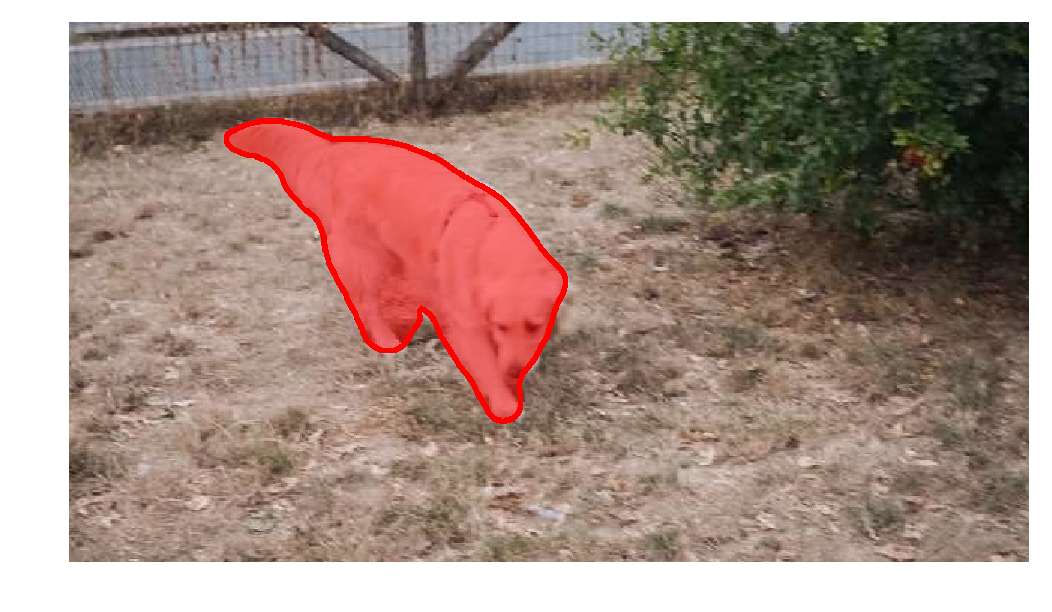
\includegraphics[trim={2.5cm 1cm 2.5cm 1cm},clip,width = 1.1in]{supp/davis16/pdf/dog/00007}
&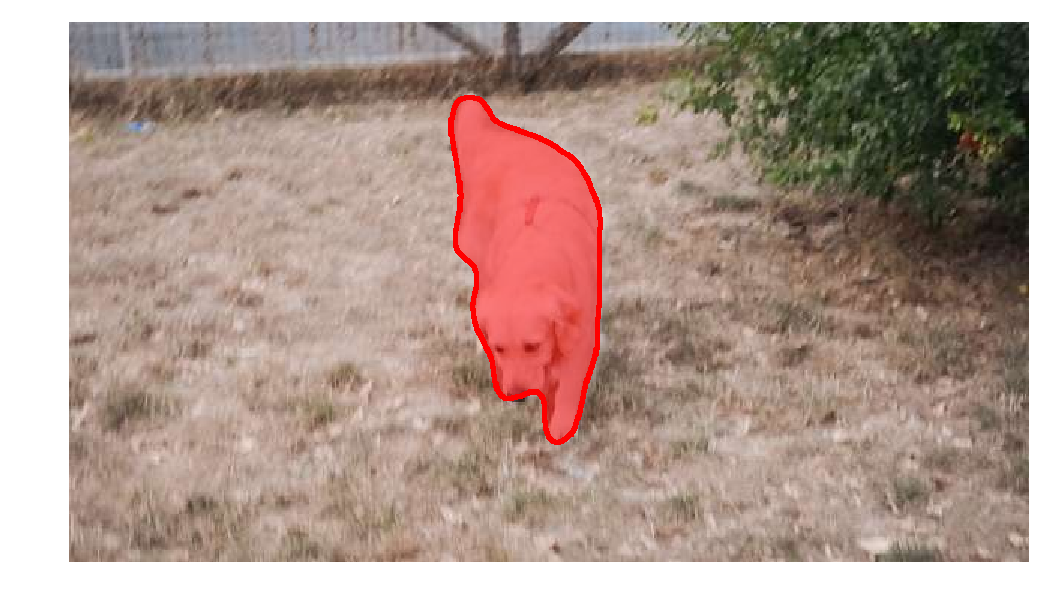
\includegraphics[trim={2.5cm 1cm 2.5cm 1cm},clip,width = 1.1in]{supp/davis16/pdf/dog/00020}
& 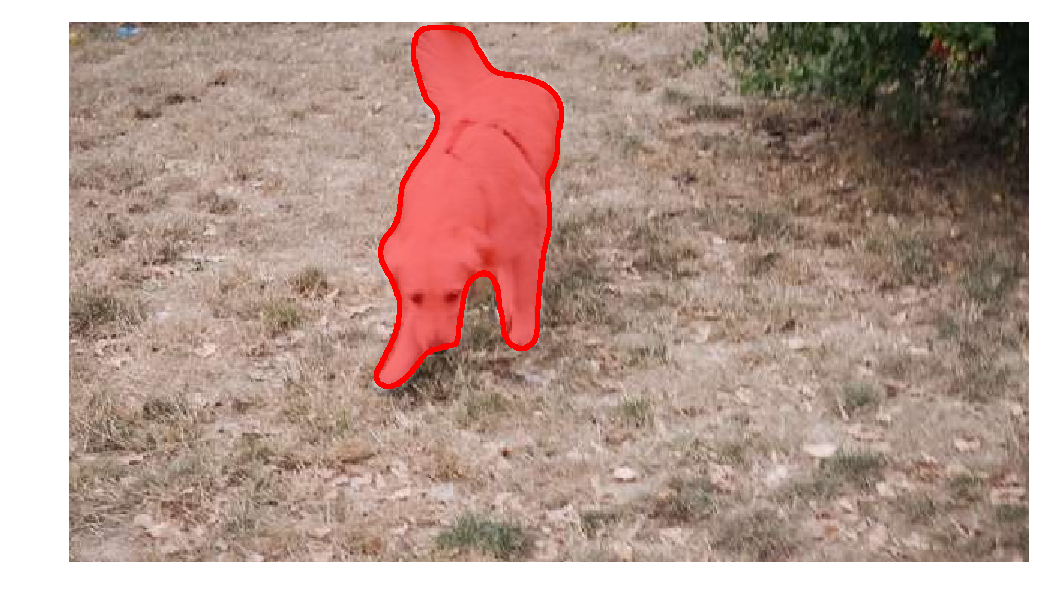
\includegraphics[trim={2.5cm 1cm 2.5cm 1cm},clip,width = 1.1in]{supp/davis16/pdf/dog/00028}
& 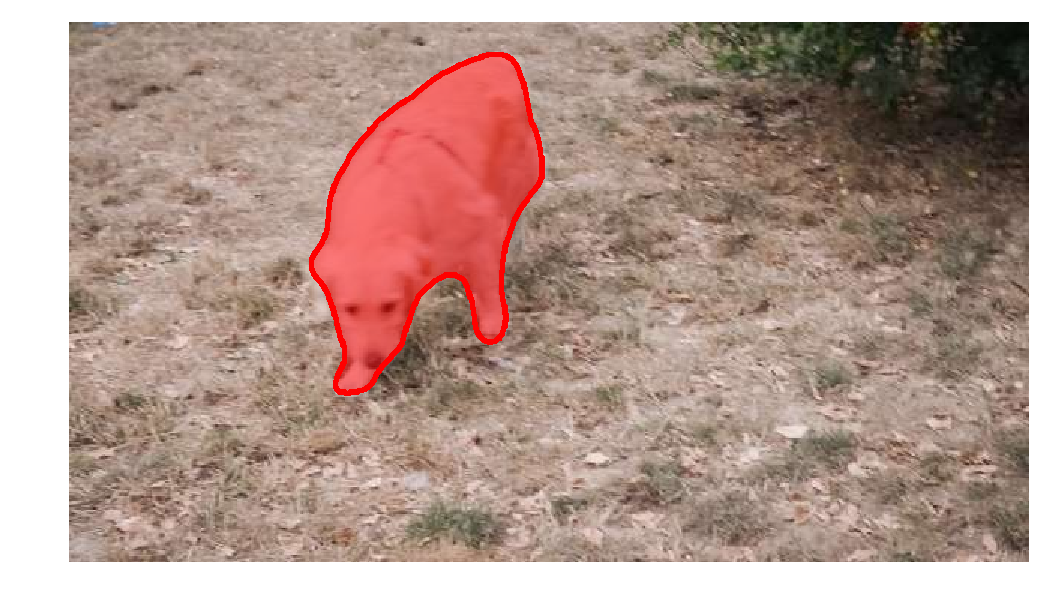
\includegraphics[trim={2.5cm 1cm 2.5cm 1cm},clip,width = 1.1in]{supp/davis16/pdf/dog/00032}
& 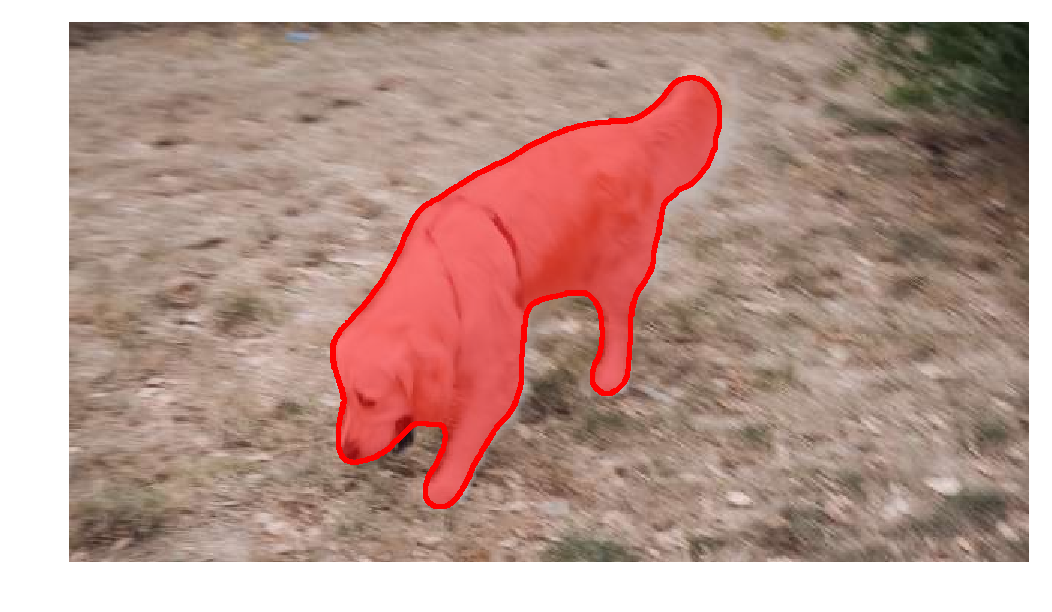
\includegraphics[trim={2.5cm 1cm 2.5cm 1cm},clip,width = 1.1in]{supp/davis16/pdf/dog/00044}
& 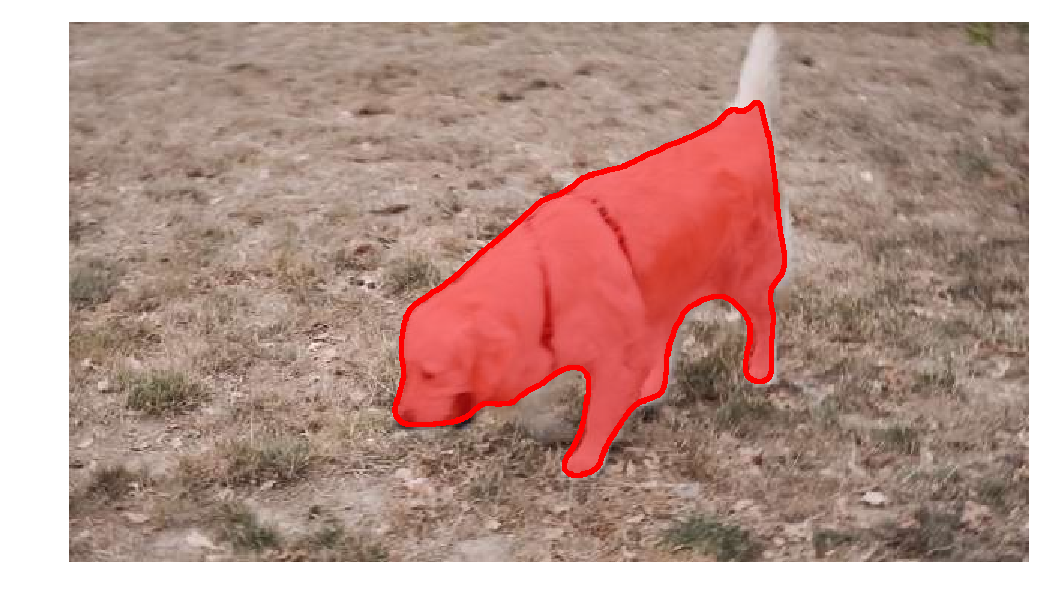
\includegraphics[trim={2.5cm 1cm 2.5cm 1cm},clip,width = 1.1in]{supp/davis16/pdf/dog/00050}
\\

\mbox{\rotatebox[x=-0.cm]{90}{\small{drift-straight}}}
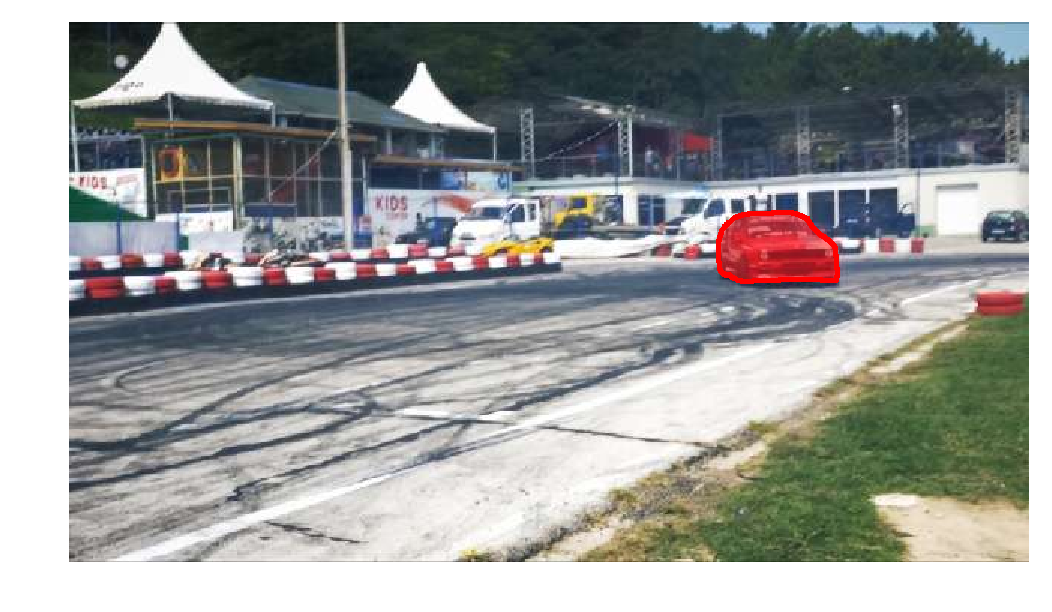
\includegraphics[trim={2.5cm 1cm 2.5cm 1cm},clip,width = 1.1in]{supp/davis16/pdf/drift-straight/00003}
&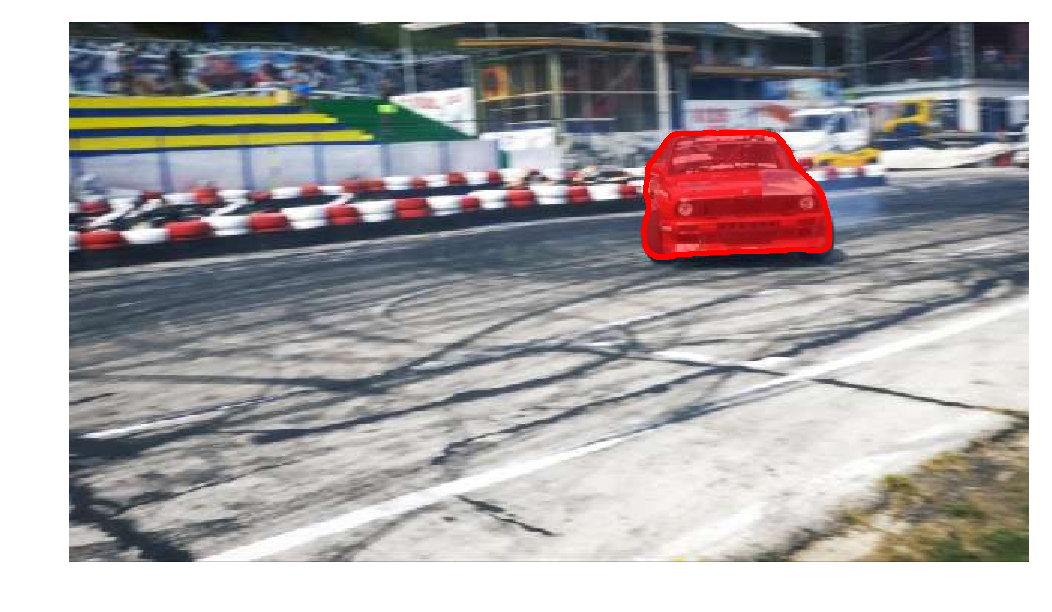
\includegraphics[trim={2.5cm 1cm 2.5cm 1cm},clip,width = 1.1in]{supp/davis16/pdf/drift-straight/00017}
& 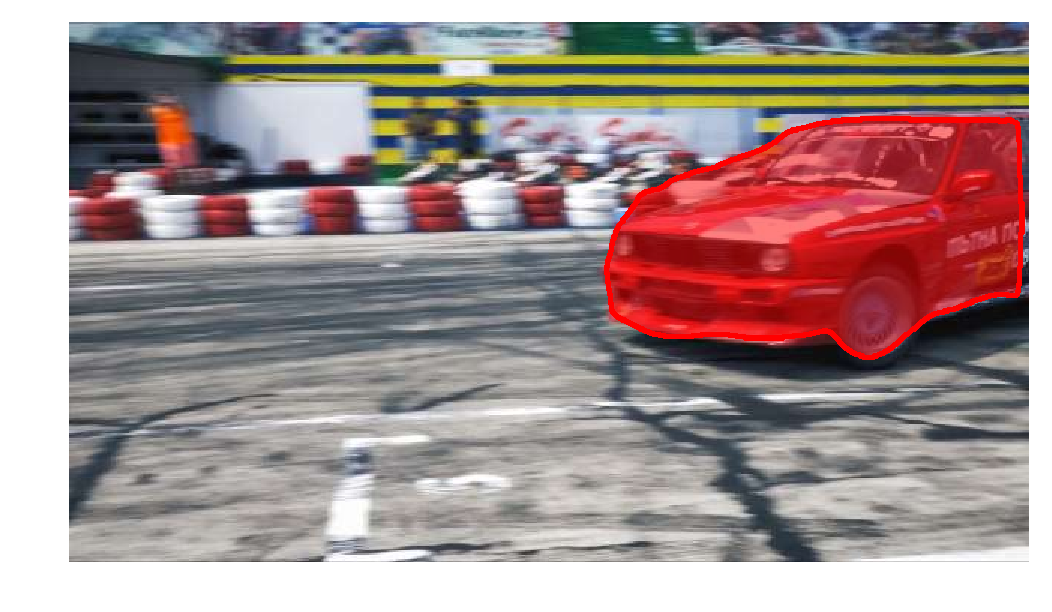
\includegraphics[trim={2.5cm 1cm 2.5cm 1cm},clip,width = 1.1in]{supp/davis16/pdf/drift-straight/00027}
& 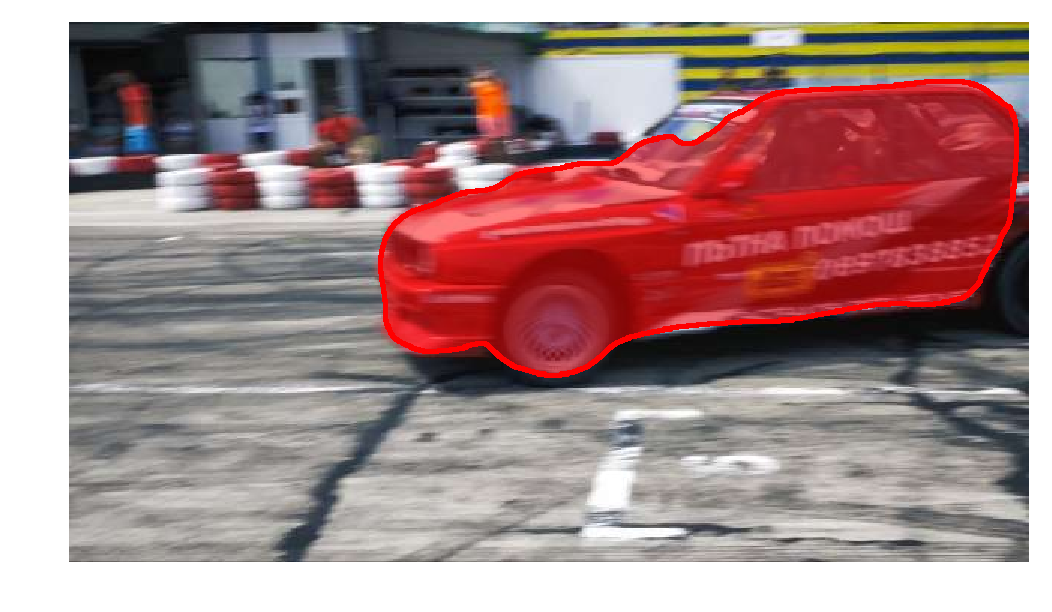
\includegraphics[trim={2.5cm 1cm 2.5cm 1cm},clip,width = 1.1in]{supp/davis16/pdf/drift-straight/00031}
& 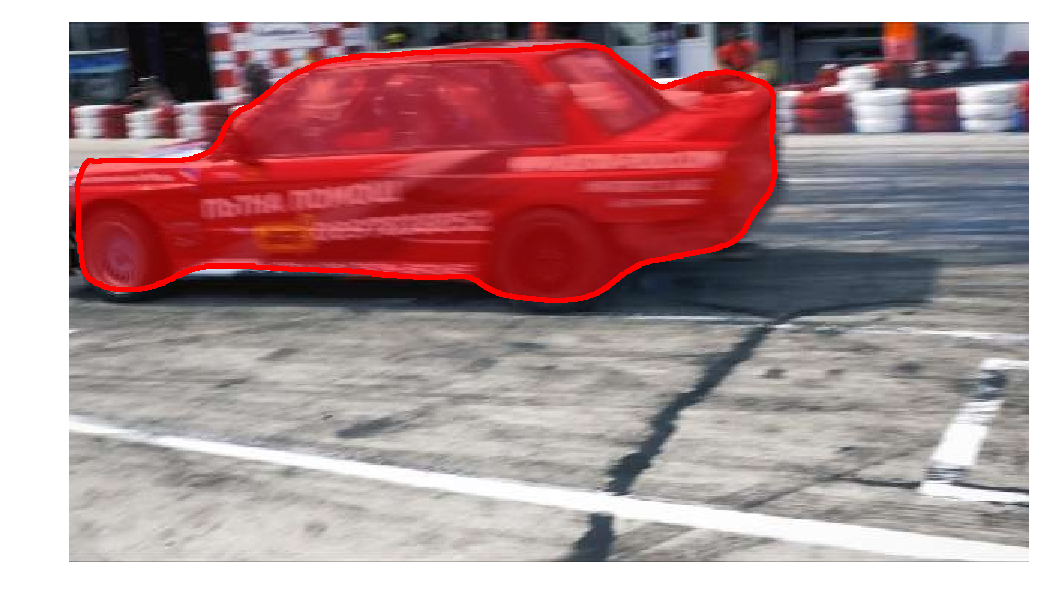
\includegraphics[trim={2.5cm 1cm 2.5cm 1cm},clip,width = 1.1in]{supp/davis16/pdf/drift-straight/00036}
& 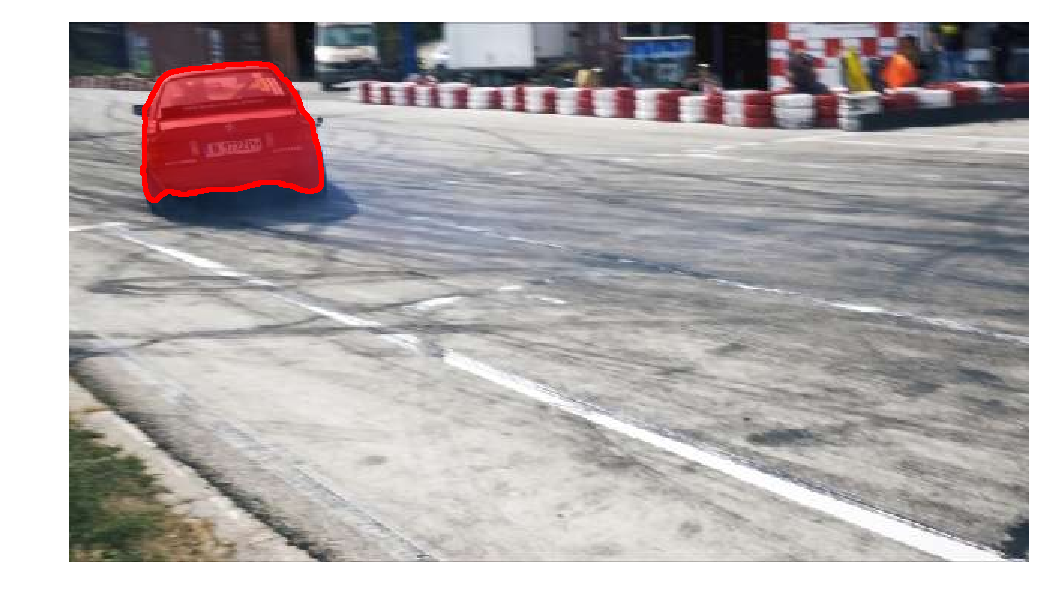
\includegraphics[trim={2.5cm 1cm 2.5cm 1cm},clip,width = 1.1in]{supp/davis16/pdf/drift-straight/00047}
\\

\mbox{\rotatebox[x=-0.55cm]{90}{\small{goat}}}
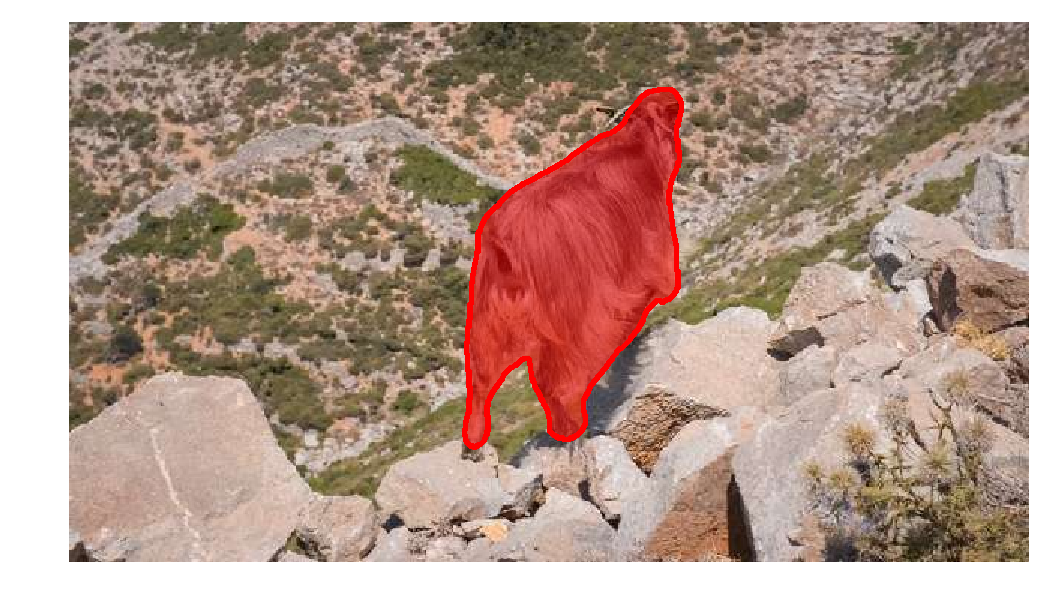
\includegraphics[trim={2.5cm 1cm 2.5cm 1cm},clip,width = 1.1in]{supp/davis16/pdf/goat/00000}
&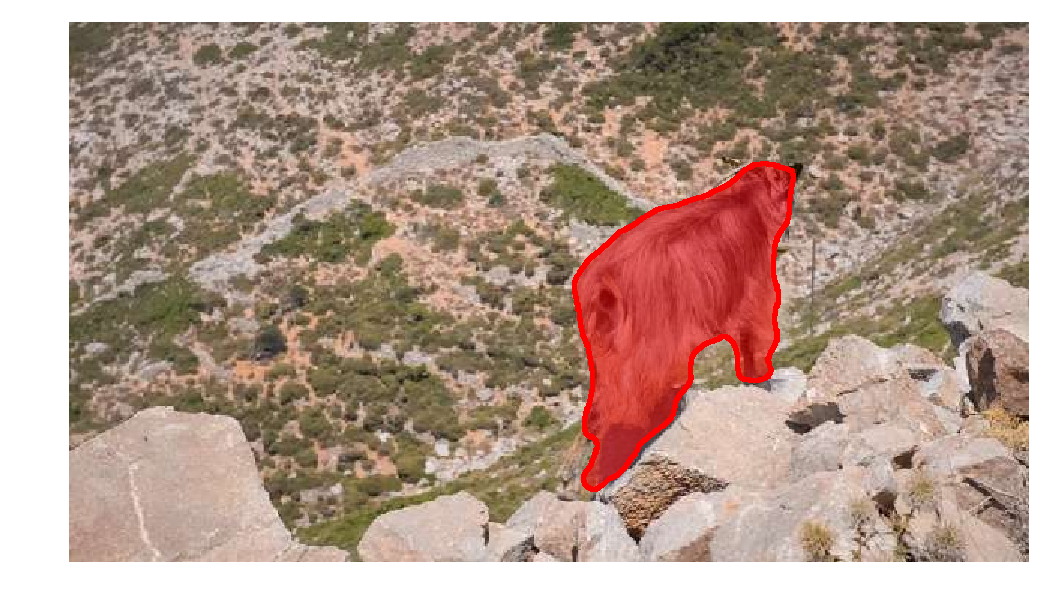
\includegraphics[trim={2.5cm 1cm 2.5cm 1cm},clip,width = 1.1in]{supp/davis16/pdf/goat/00014}
& 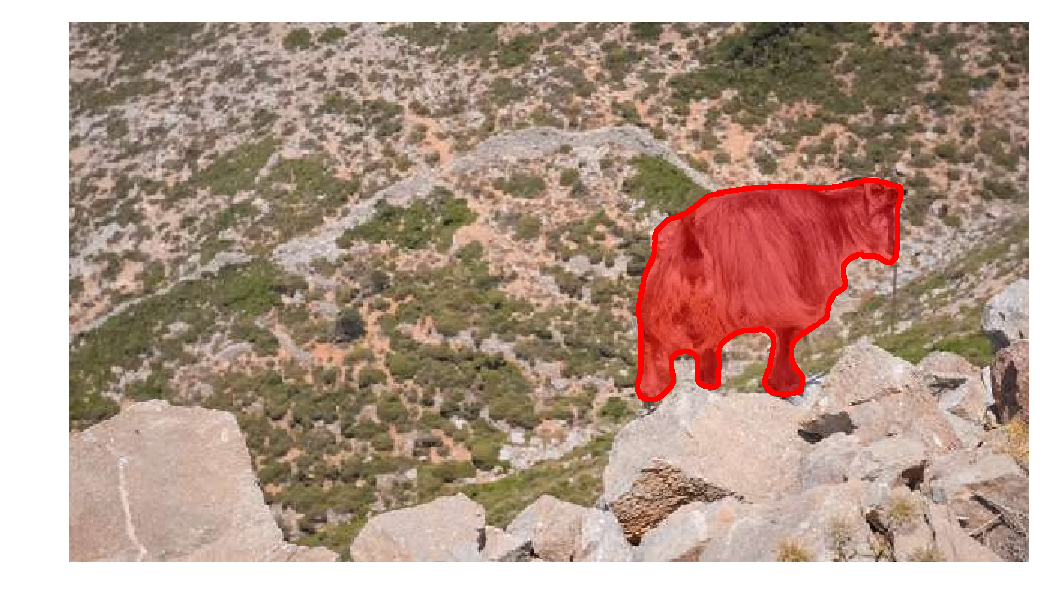
\includegraphics[trim={2.5cm 1cm 2.5cm 1cm},clip,width = 1.1in]{supp/davis16/pdf/goat/00025}
& 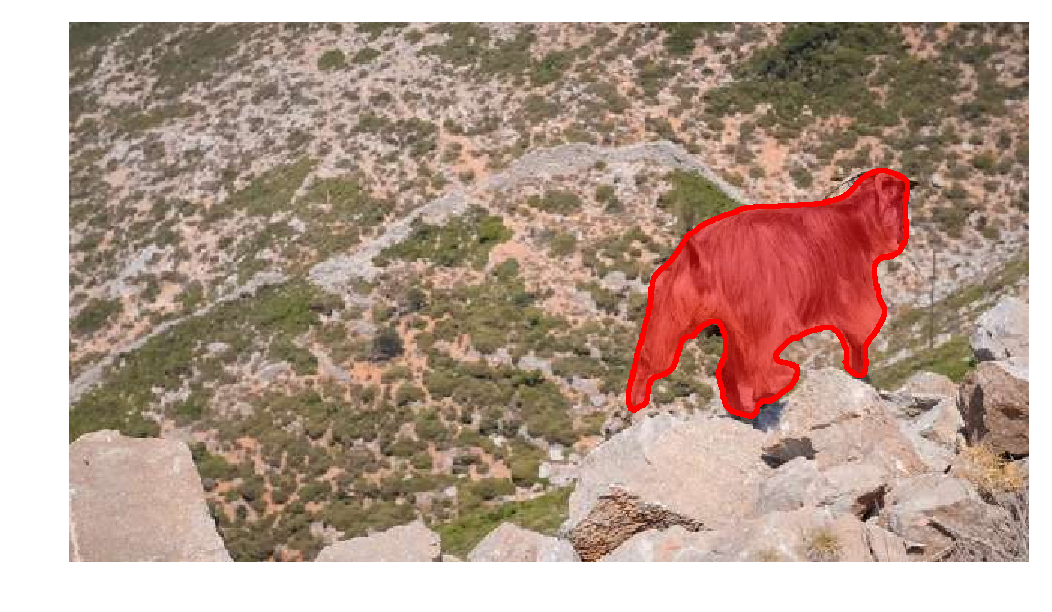
\includegraphics[trim={2.5cm 1cm 2.5cm 1cm},clip,width = 1.1in]{supp/davis16/pdf/goat/00036}
& 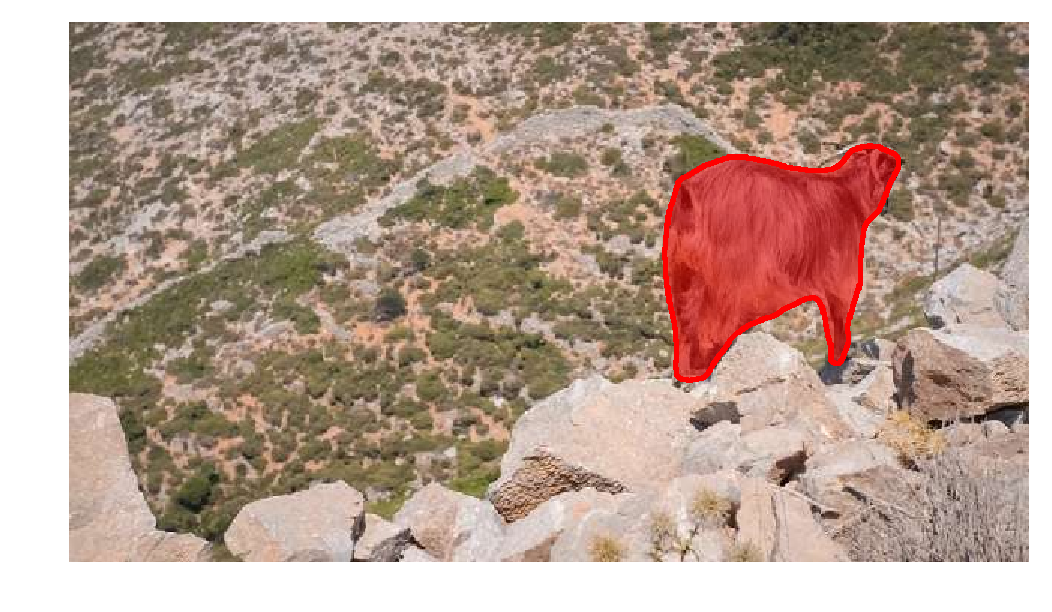
\includegraphics[trim={2.5cm 1cm 2.5cm 1cm},clip,width = 1.1in]{supp/davis16/pdf/goat/00045}
& 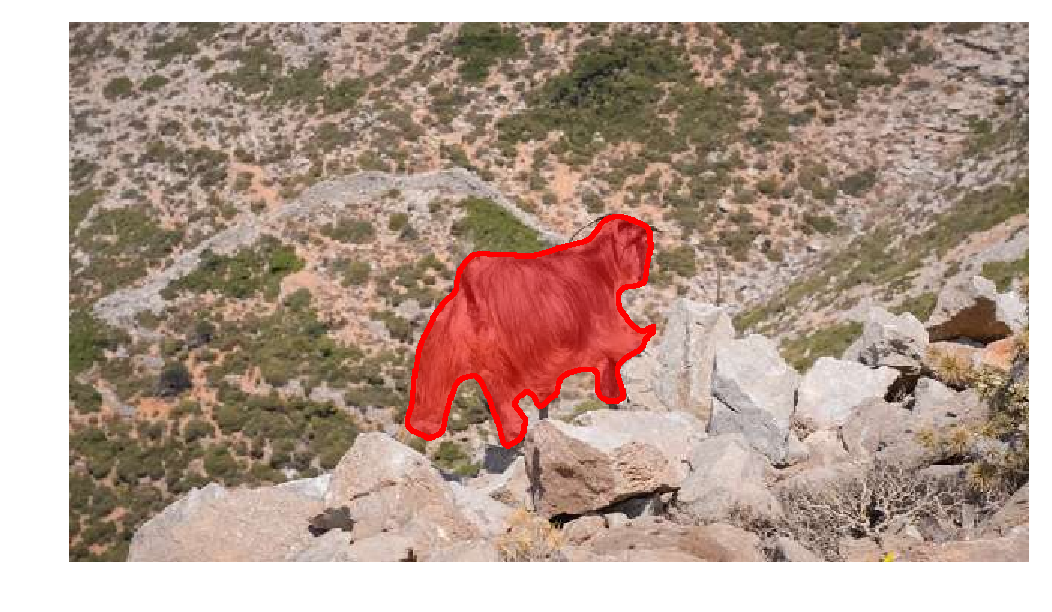
\includegraphics[trim={2.5cm 1cm 2.5cm 1cm},clip,width = 1.1in]{supp/davis16/pdf/goat/00067}
\\


\mbox{\rotatebox[x=-0.55cm]{90}{\small{Libby}}}
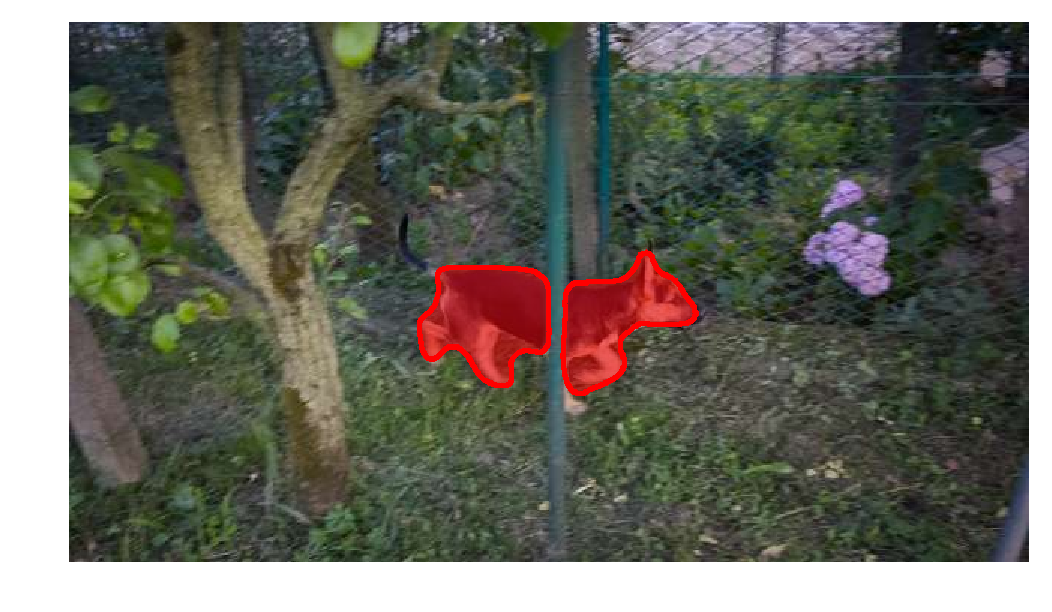
\includegraphics[trim={2.5cm 1cm 2.5cm 1cm},clip,width = 1.1in]{supp/davis16/pdf/libby/00000}
&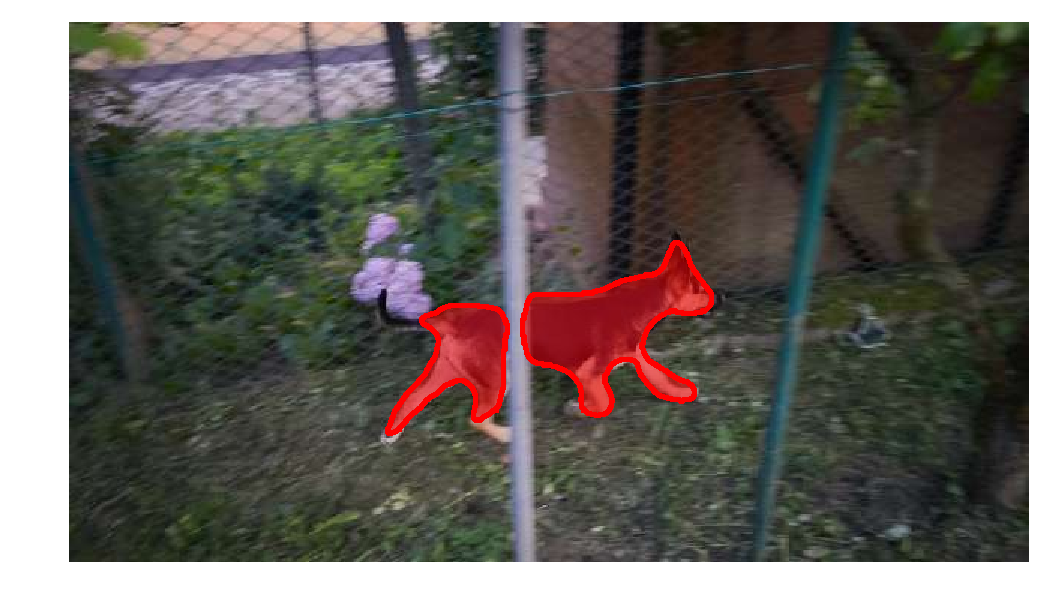
\includegraphics[trim={2.5cm 1cm 2.5cm 1cm},clip,width = 1.1in]{supp/davis16/pdf/libby/00016}
& 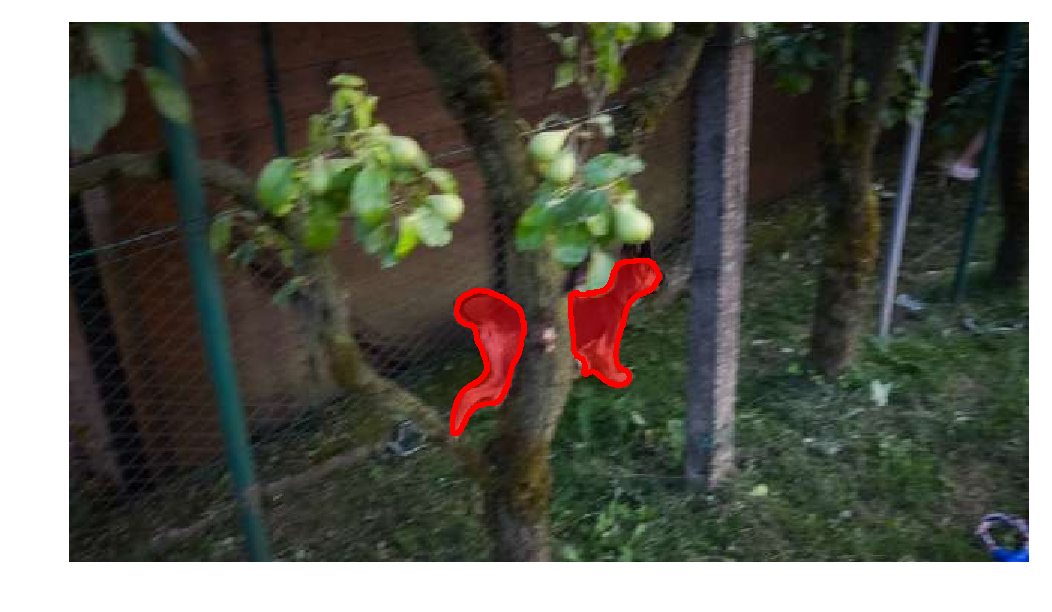
\includegraphics[trim={2.5cm 1cm 2.5cm 1cm},clip,width = 1.1in]{supp/davis16/pdf/libby/00035}
& 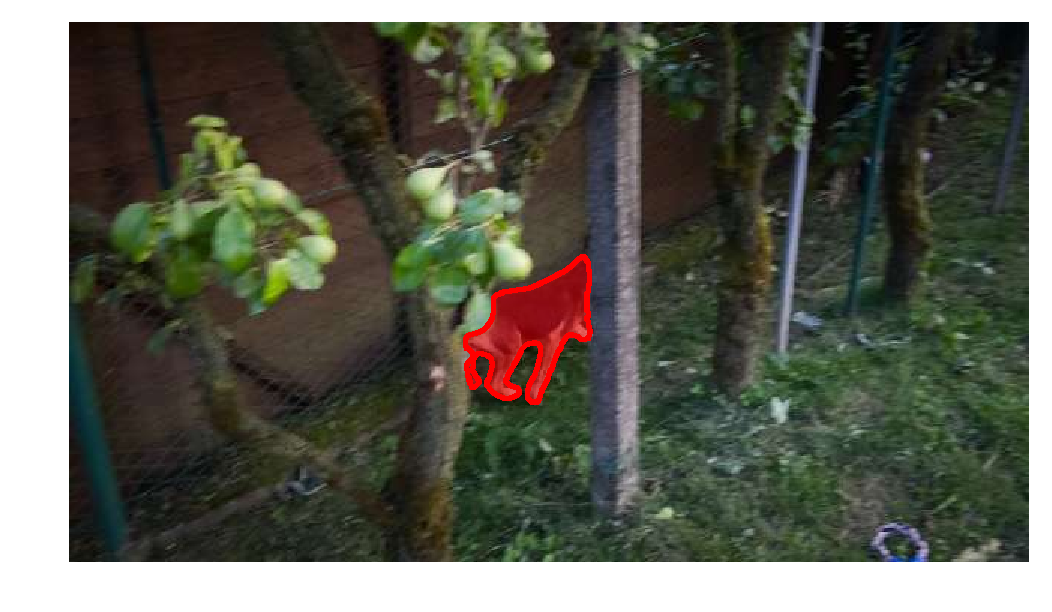
\includegraphics[trim={2.5cm 1cm 2.5cm 1cm},clip,width = 1.1in]{supp/davis16/pdf/libby/00039}
& 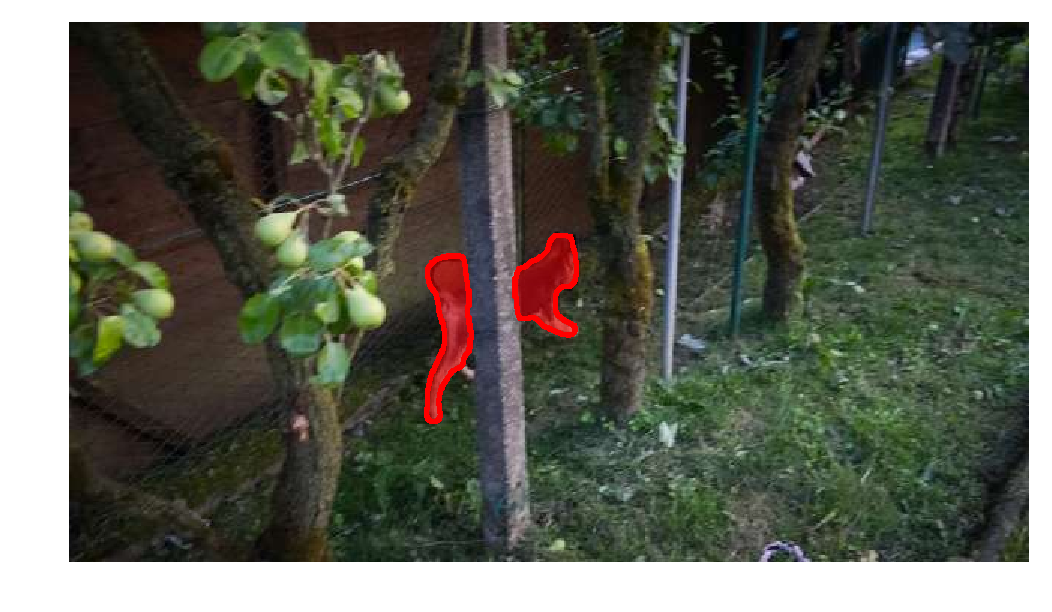
\includegraphics[trim={2.5cm 1cm 2.5cm 1cm},clip,width = 1.1in]{supp/davis16/pdf/libby/00045}
& 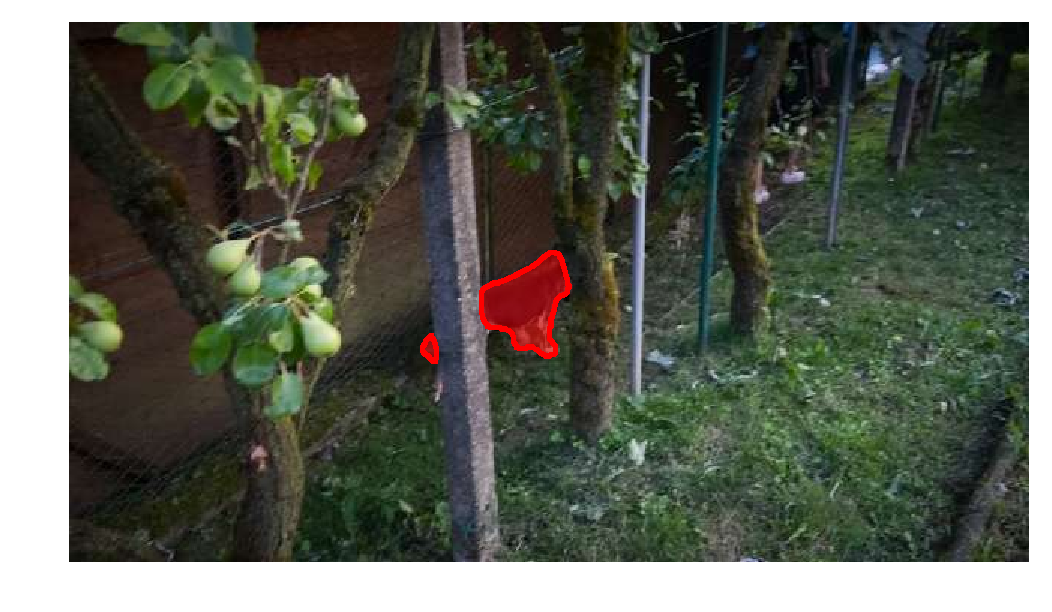
\includegraphics[trim={2.5cm 1cm 2.5cm 1cm},clip,width = 1.1in]{supp/davis16/pdf/libby/00048}
\\

\mbox{\rotatebox[x=-0.cm]{90}{\scriptsize{motocross-jump}}}
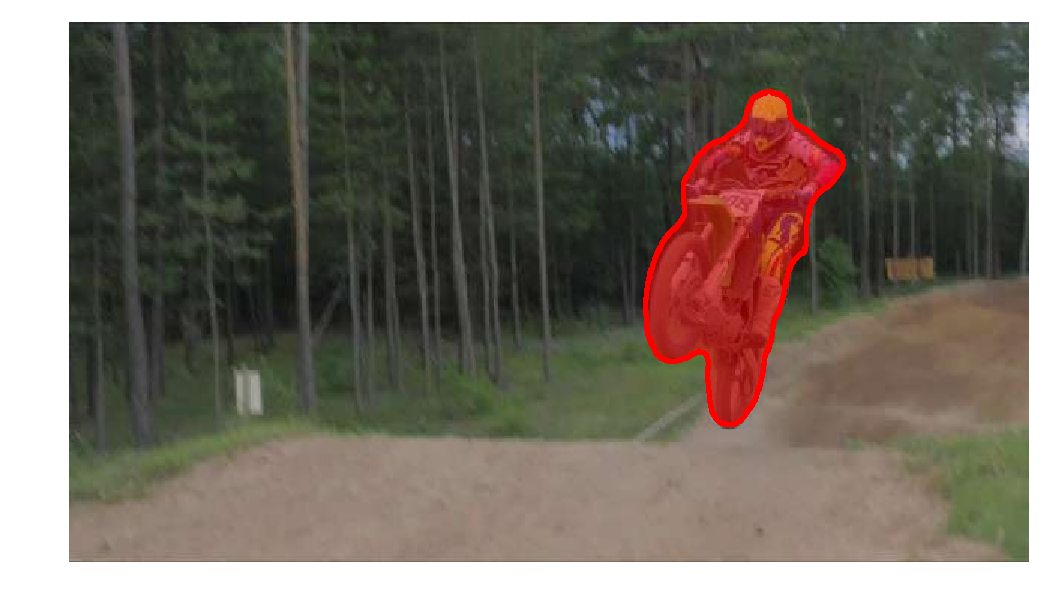
\includegraphics[trim={2.5cm 1cm 2.5cm 1cm},clip,width = 1.1in]{supp/davis16/pdf/motocross-jump/00004}
&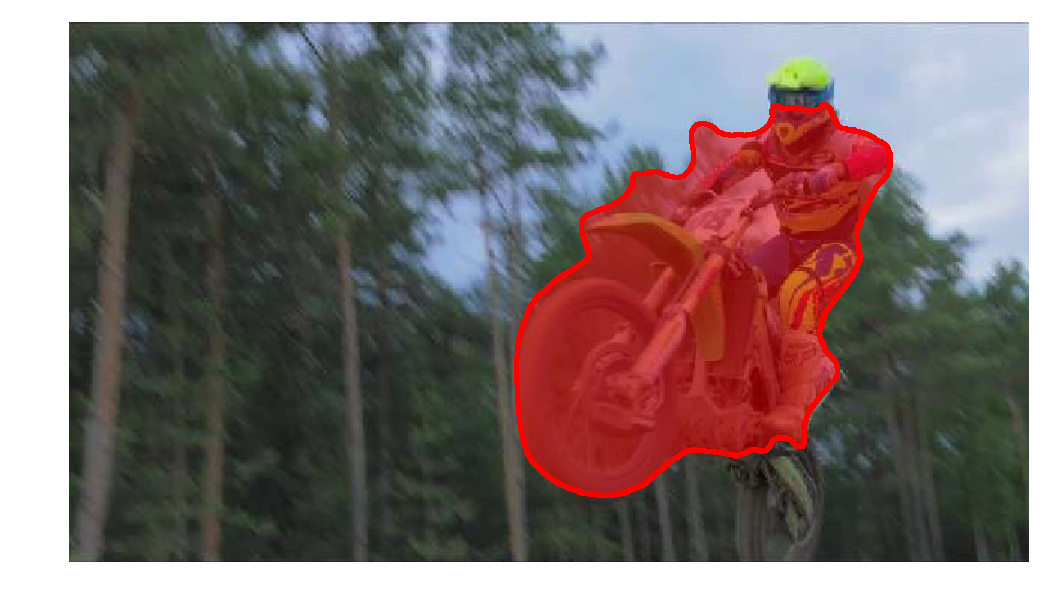
\includegraphics[trim={2.5cm 1cm 2.5cm 1cm},clip,width = 1.1in]{supp/davis16/pdf/motocross-jump/00010}
& 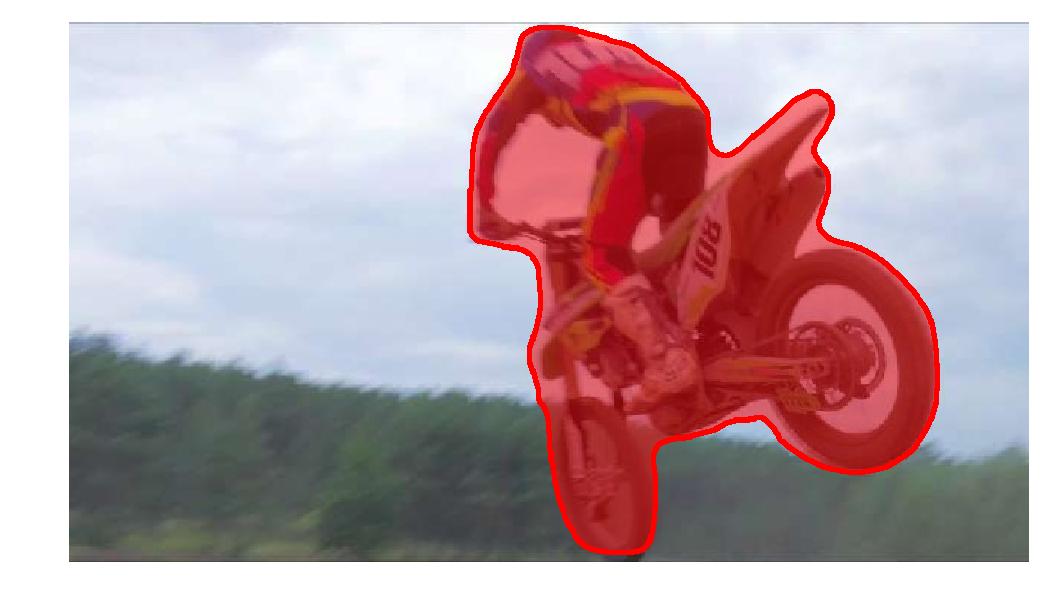
\includegraphics[trim={2.5cm 1cm 2.5cm 1cm},clip,width = 1.1in]{supp/davis16/pdf/motocross-jump/00027}
& 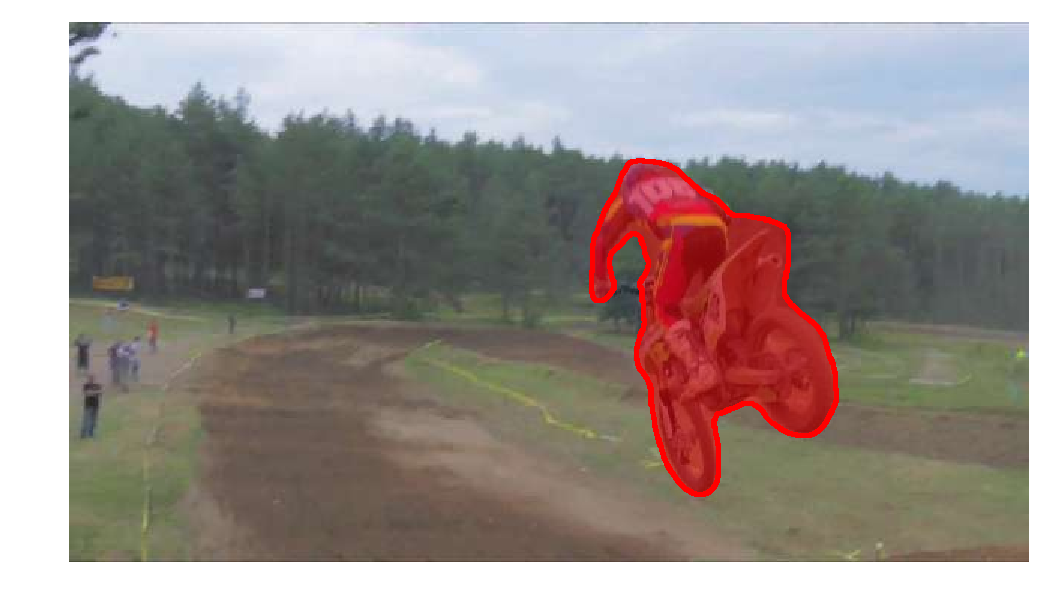
\includegraphics[trim={2.5cm 1cm 2.5cm 1cm},clip,width = 1.1in]{supp/davis16/pdf/motocross-jump/00033}
& 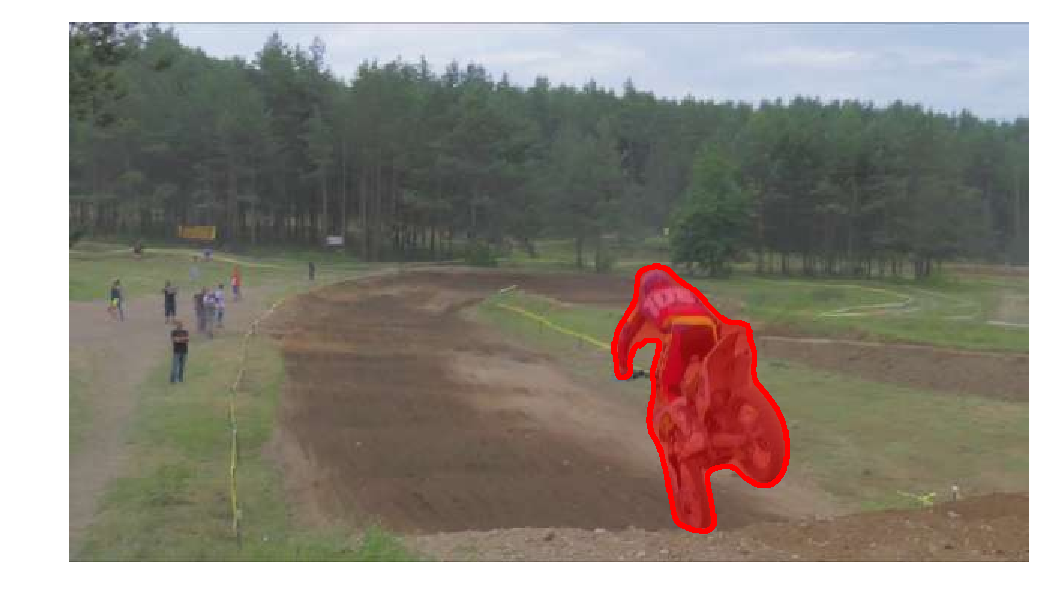
\includegraphics[trim={2.5cm 1cm 2.5cm 1cm},clip,width = 1.1in]{supp/davis16/pdf/motocross-jump/00037}
& 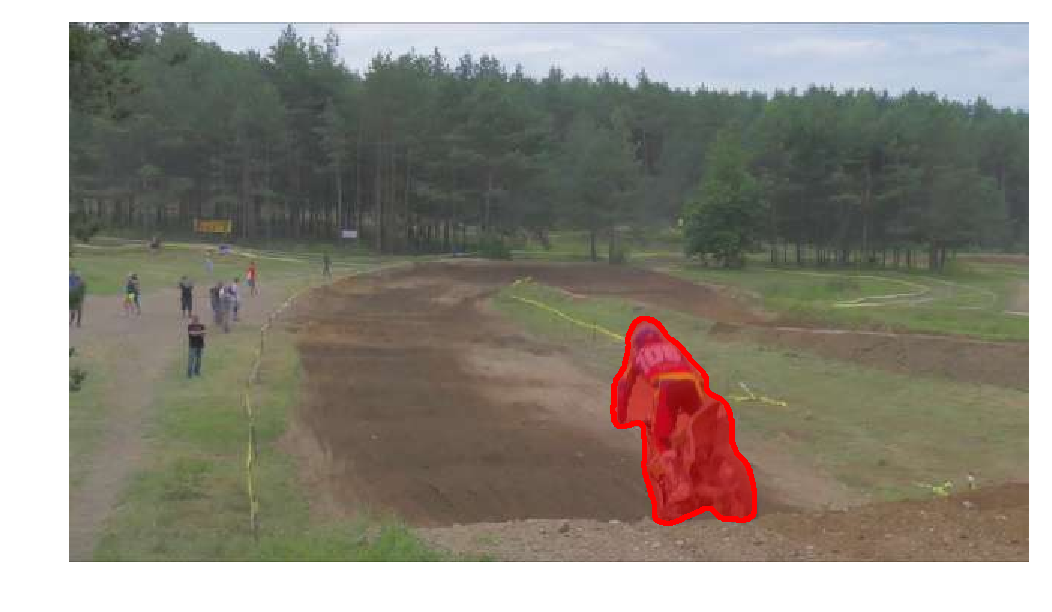
\includegraphics[trim={2.5cm 1cm 2.5cm 1cm},clip,width = 1.1in]{supp/davis16/pdf/motocross-jump/00039}
\\


\mbox{\rotatebox[x=-0.55cm]{90}{\small{parkour}}}
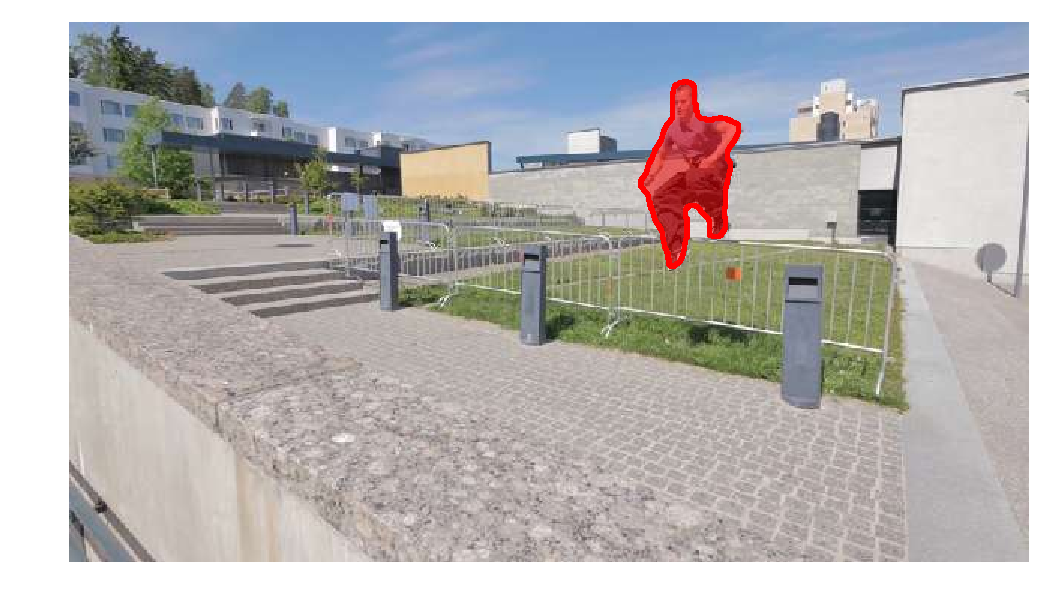
\includegraphics[trim={2.5cm 1cm 2.5cm 0.5cm},clip,width = 1.1in]{supp/davis16/pdf/parkour/00000}
&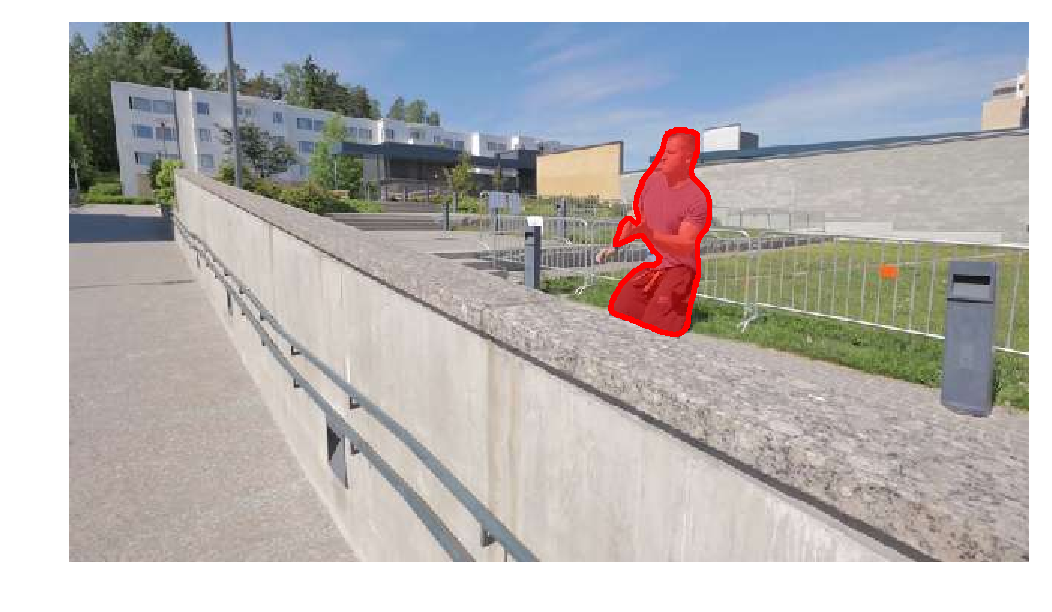
\includegraphics[trim={2.5cm 1cm 2.5cm 0.5cm},clip,width = 1.1in]{supp/davis16/pdf/parkour/00016}
& 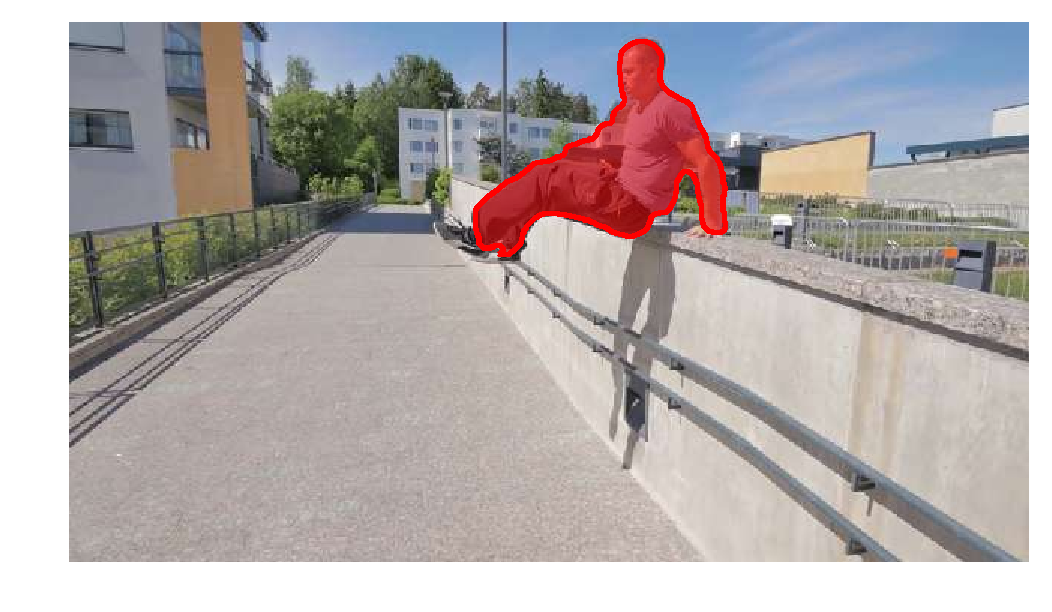
\includegraphics[trim={2.5cm 1cm 2.5cm 0.5cm},clip,width = 1.1in]{supp/davis16/pdf/parkour/00033}
& 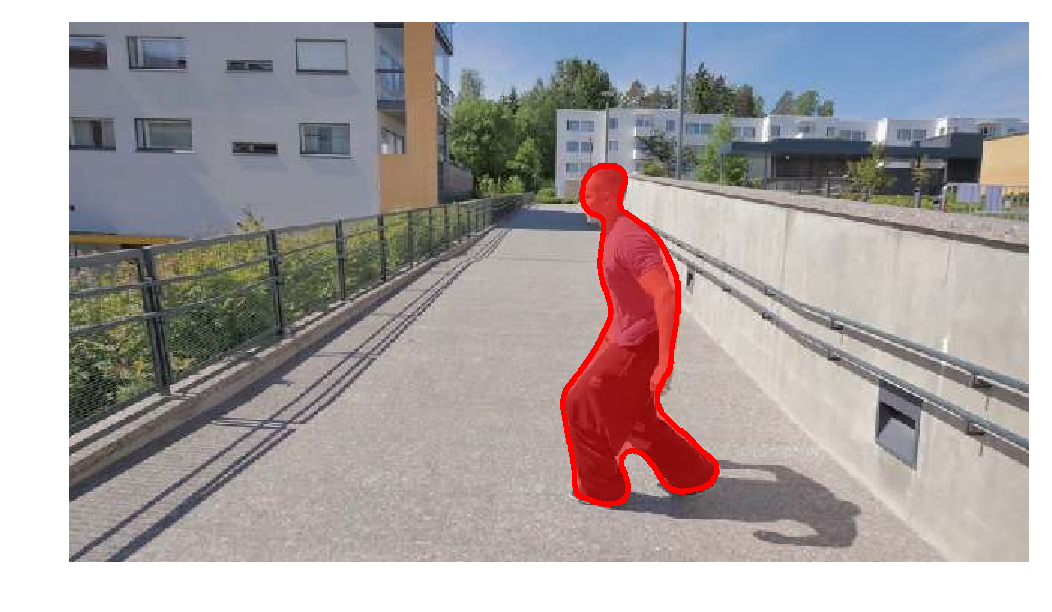
\includegraphics[trim={2.5cm 1cm 2.5cm 0.5cm},clip,width = 1.1in]{supp/davis16/pdf/parkour/00043}
& 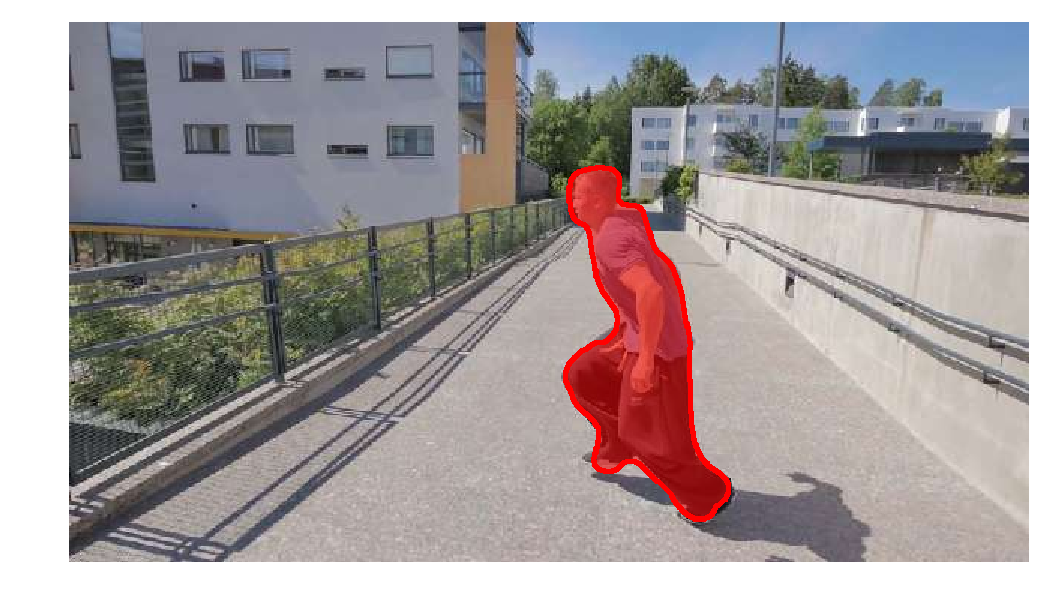
\includegraphics[trim={2.5cm 1cm 2.5cm 0.5cm},clip,width = 1.1in]{supp/davis16/pdf/parkour/00047}
& 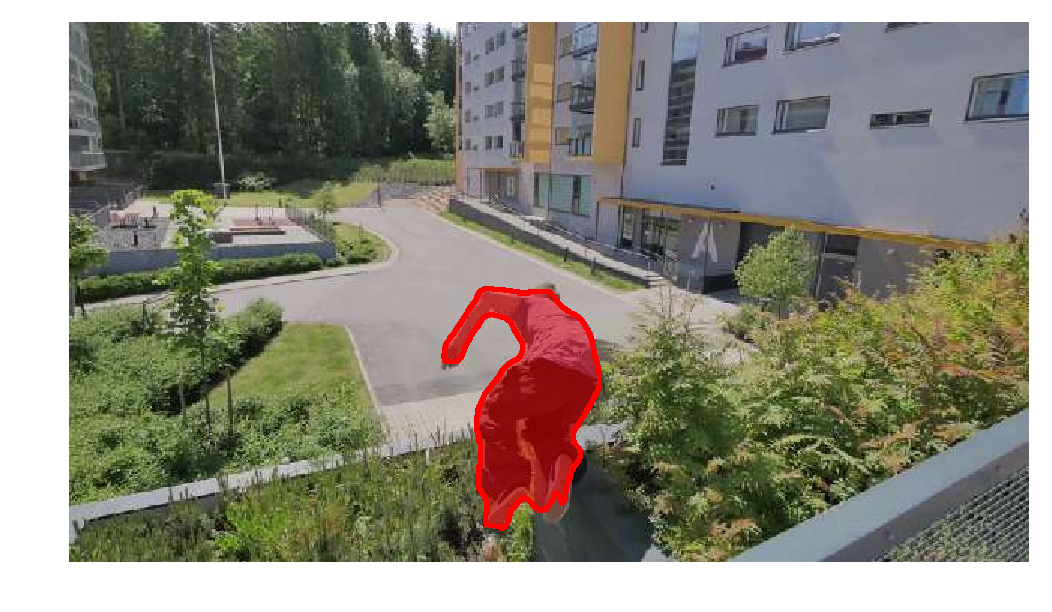
\includegraphics[trim={2.5cm 1cm 2.5cm 0.5cm},clip,width = 1.1in]{supp/davis16/pdf/parkour/00090}
\\
\mbox{\rotatebox[x=-0.0cm]{90}{\small{Gold-Fish}}}
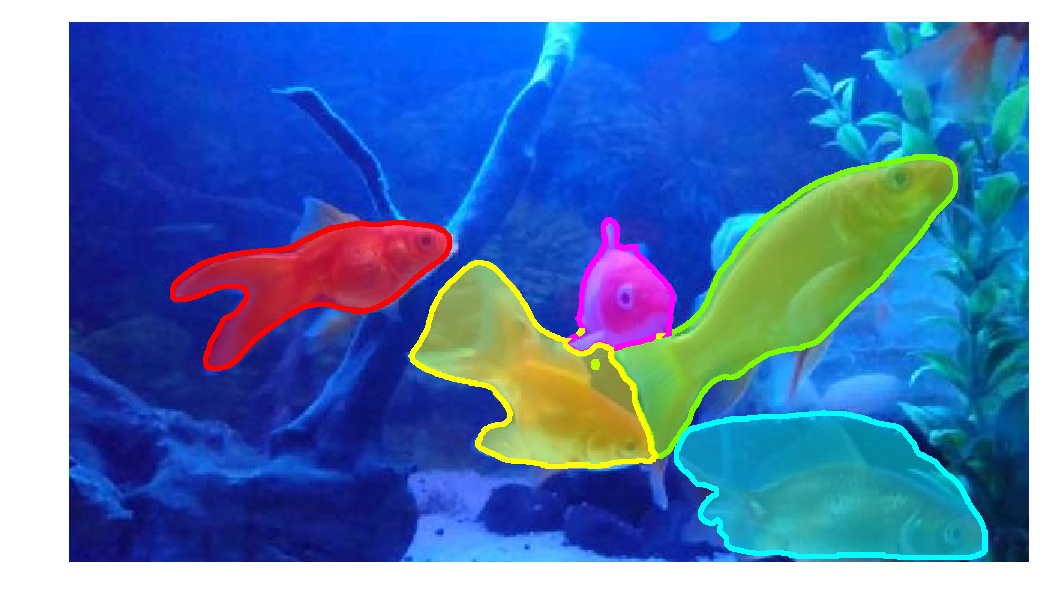
\includegraphics[trim={2.5cm 1cm 2.5cm 1cm},clip,width = 1.1in]{img/davis16/pdf/gold-fish/00003}
&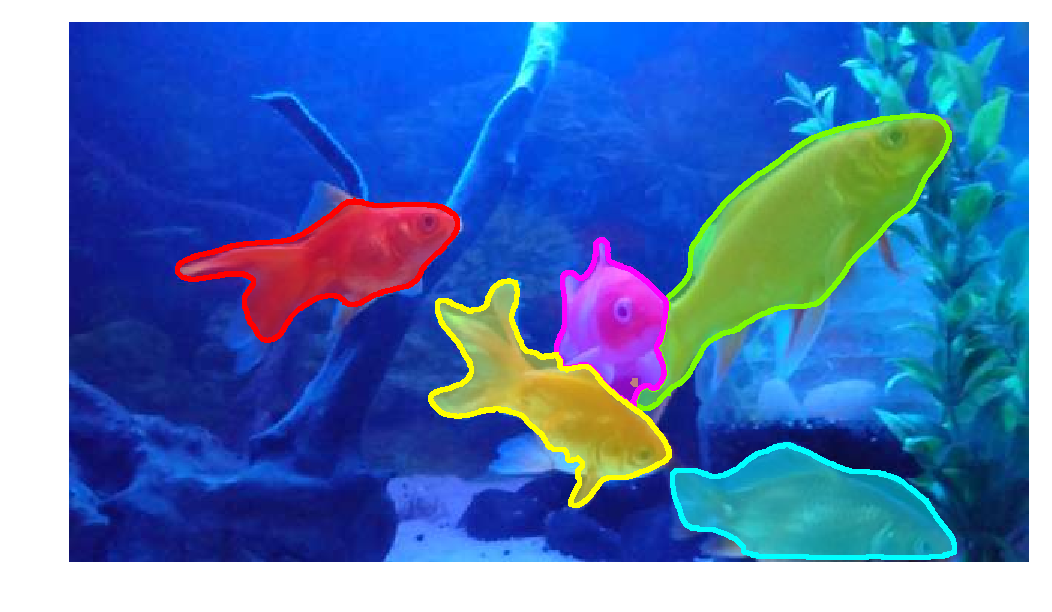
\includegraphics[trim={2.5cm 1cm 2.5cm 1cm},clip,width = 1.1in]{img/davis16/pdf/gold-fish/00012}
& 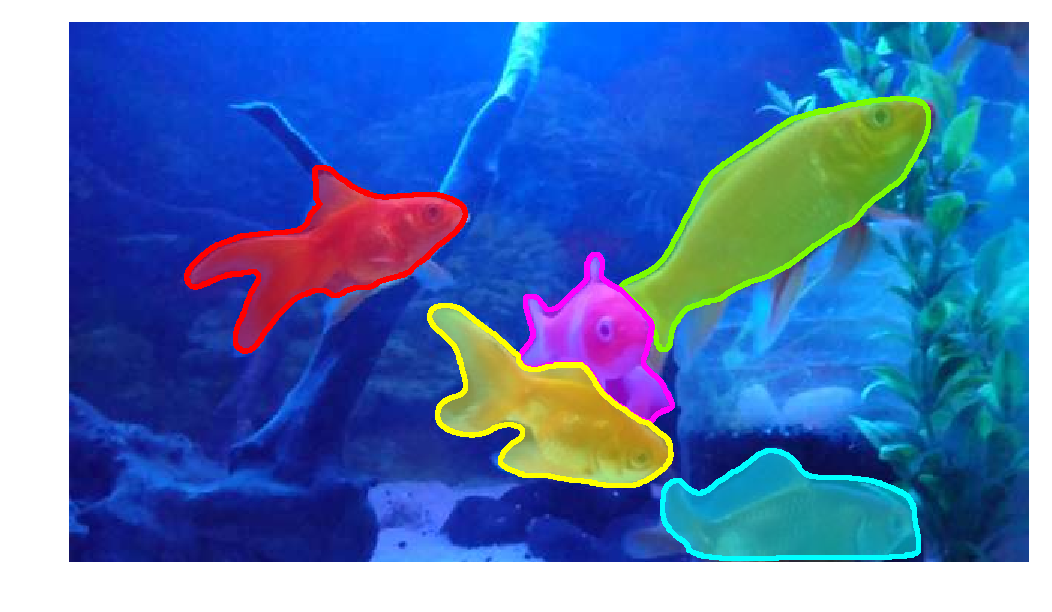
\includegraphics[trim={2.5cm 1cm 2.5cm 1cm},clip,width = 1.1in]{img/davis16/pdf/gold-fish/00020}
& 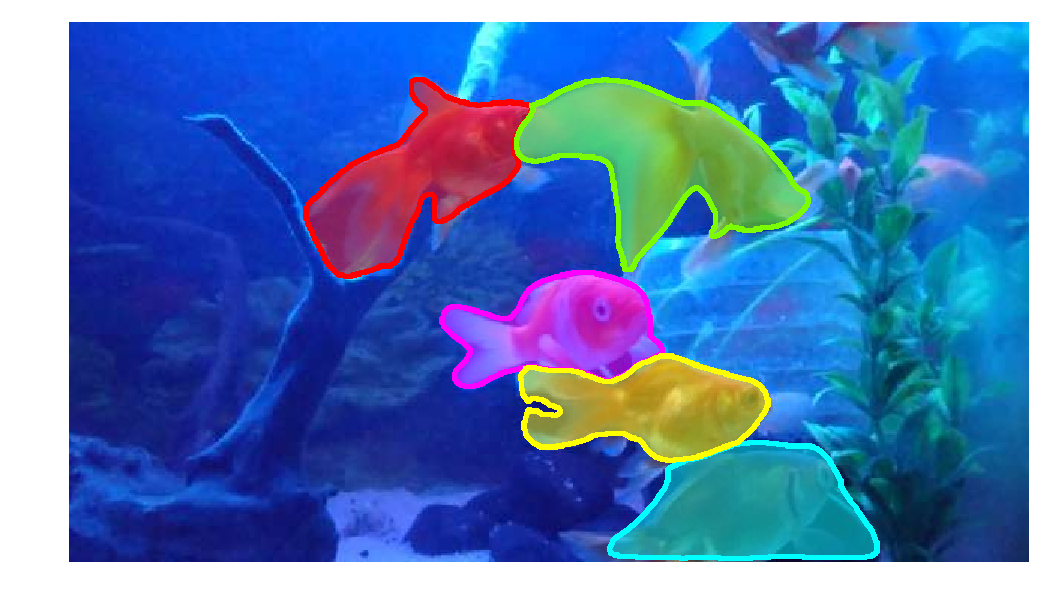
\includegraphics[trim={2.5cm 1cm 2.5cm 1cm},clip,width = 1.1in]{img/davis16/pdf/gold-fish/00054}
& 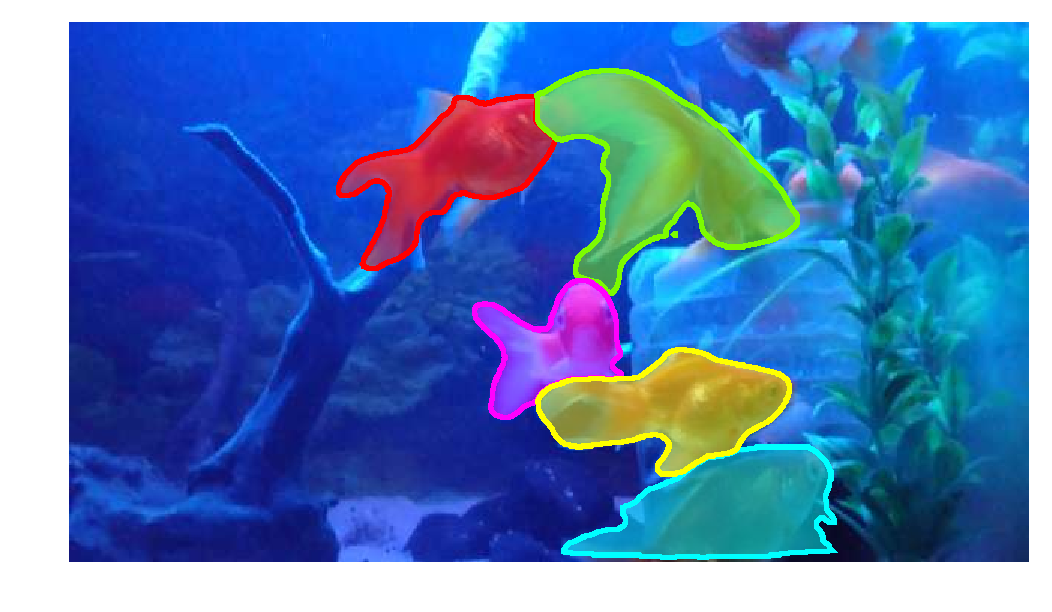
\includegraphics[trim={2.5cm 1cm 2.5cm 1cm},clip,width = 1.1in]{img/davis16/pdf/gold-fish/00060}
& 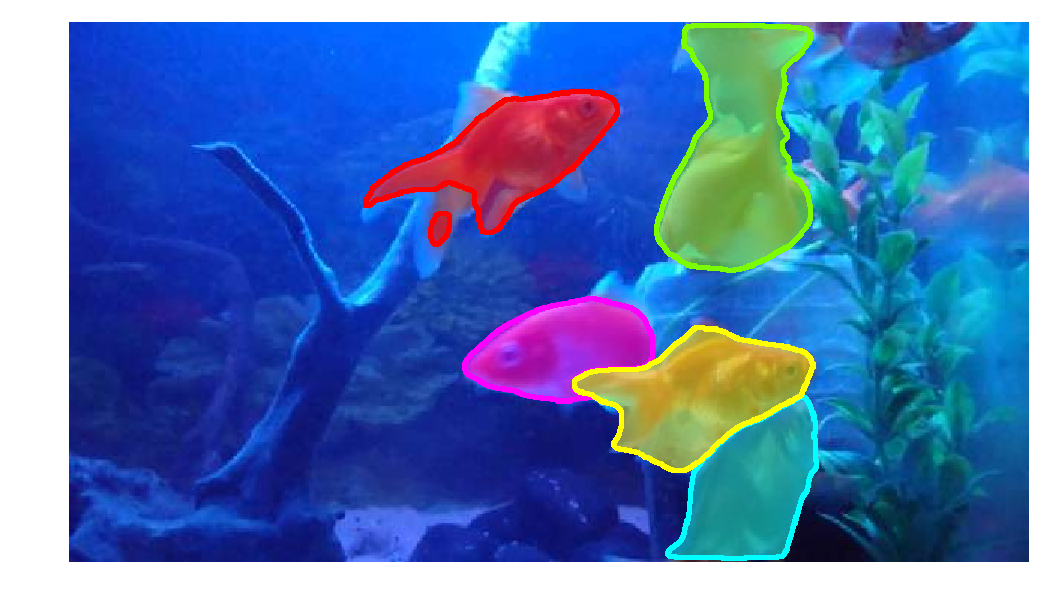
\includegraphics[trim={2.5cm 1cm 2.5cm 1cm},clip,width = 1.1in]{img/davis16/pdf/gold-fish/00070}
\\


\end{tabular}

\caption{\bd{Qualitative results} of our method for sequences belonging to both object tracking and video object segmentation benchmarks.
\emph{Basketball} and \emph{Nature} are from VOT-2018~\cite{VOT2018}; \emph{Car-Shadow} is from DAVIS-2016~\cite{perazzi2016benchmark}; \emph{Dogs-Jump} and \emph{Pigs} are from DAVIS-2017~\cite{pont2017davis}.
Multiple masks are obtained from different inferences (with different initialisations).	
}	
\label{fig:davis16}
\vspace{-0.5cm}
\end{figure*}
